% ---------------------------------------------------------------------------
% Body of the ATTRIB camera-ready: the AISTATS 2027 submission, in full.
% ---------------------------------------------------------------------------
\maketitle

% blank footnote (no mark); the pdfborder setting stops hyperref drawing an empty link box in the margin
{\hypersetup{pdfborder={0 0 0}}\blfootnote{DISTRIBUTION STATEMENT A. Approved for public release. Distribution is unlimited.}}

\begin{abstract}
Scientists often want to explain why an outcome is different in two groups. For instance, would two hospitals (the groups) with different mortality rates (the outcome) fare more similarly if they treated the same patients? What if they followed the same care protocols? The Oaxaca--Blinder decomposition (OBD) is a standard tool to answer these questions. It is well known that the OBD requires choosing one of the groups as a reference point, and the numerical answer can vary with the reference. To the best of our knowledge, we are the first to show that the choice of reference groups can produce contradictory conclusions; for example, choosing one reference might imply the two hospitals achieve more-similar mortality rates when they treat the same patients, and the other reference might imply less-similar rates. We show these reversals can happen in both real and simulated data. Our empirical exercises show that extending the OBD to more-complex regression models, including a pretrained transformer, does not eliminate these reversals, and can even worsen their prevalence. Our theoretical results further establish that these conclusion reversals are not entirely driven by model misspecification, finite-sample concerns, or knife-edge parameter choices.
\end{abstract}

% Main sections (same files and order as AISTATS27/OBD_AISTATS.tex)
\section{Introduction}
\label{sec:intro}
% Para 1: set up data analysis problem
As a motivating example, suppose a data scientist notices that mortality rates are noticeably higher at Hospital $H$ than at Hospital $K$.
She knows the medical literature links many risk factors ($X$), such as high blood pressure, to mortality ($Y$).
The observed differences in mortality could be due to differences in these risk factors between the two groups of patients (distribution of $X$) or to differences in how well each hospital manages these risk factors (distribution of $Y \mid X$).
If she can figure out how much each of these components contributes to the difference in mortality rates, Hospital $H$ may be able to improve patient outcomes.
How can she use the available information to form hypotheses about what drives the difference in mortality?

% Para 2: Connect to ML / AI and reject existing explainability tools
The modern explainability literature in machine learning boasts a bevy of methods for attributing outcome behavior to covariates \citep{Dwivedi2023}.
These include Shapley values \citep{Shapley1953, Lundberg2017, chen2025shapley}, Functional ANOVA \citep{stone1994, hooker2004discovering, hookerGeneralizedFunctionalANOVA2007, lengerich2020purifying, fumagalli2025fanova}, Accumulated Local Effects \citep{apley2020}, and partial dependence plots \citep{friedman2001greedy, liu2025trees}.
However, such methods are not designed to answer this data scientist's question.
They attribute variation in outcomes within a single population to the covariates, holding the conditional distribution $Y | X$ fixed.
But, the data scientist is interested in why an outcome varies between two populations, where the $Y | X$ may vary.
See \cref{appendix:xAI} for more discussion on why these methods do not solve the data scientist's question.
% For example, a Shapley value analysis of $Y \mid X$ might suggest that that patients with severe chronic conditions have higher mortality in each of hospital $H$ and $K$. 
% But if hospitals $H$ and $K$ both treat similar patient populations, chronic health conditions cannot explain why mortality rates differ between them.

% Part 3: Introduce OBD
Instead, the data scientist might adopt the Oaxaca--Blinder decomposition (OBD), which attributes disparities between two groups to $X$ and $Y \mid X$. 
The OBD was developed for linear models \citep{oaxaca1973,blinder1973} and remains widely used in this form --- e.g., to analyze wage gaps \citep{paradaContzen2025}, educational attainment differences \citep{barhaim2023}, and health disparities \citep{cartwright2021,elder2026political}. Recent work has explored pairing the OBD with flexible functional decompositions \citep{quintero2025,bach2024heterogeneity,quintas2024multiply,mao2025double,flachaire2025decomposing}; see \cref{appendix:obd_generalized} for more discussion of these methods.

%Modern machine learning explainability tools seem well-suited for this task.
%Flexible regression models like neural networks and random forests are widely used to fit distributions $Y \mid X$, and functional decomposition methods like Accumulated Local Effects (ALE) \textcolor{red}{TODO: cite} and functional ANOVA (FANOVA) \textcolor{red}{TODO: cite} help practitioners gain fine-grained understanding of these models.
%And use of these tools has been previously studied for analyzing differences between characteristics of two populations as in the example above \textcolor{red}{TODO: cite our workshop paper}.
%Under the hood, however, such analysis methods fall back to generalizations of the Oaxaca--Blinder decomposition (OBD)\footnote{Sometimes referred to as the Kitagawa--Oaxaca--Blinder (KOB) decomposition \citep{kitagawa1955}} \citep{oaxaca1973,blinder1973}, which analyzes disparities between groups by assuming a linear model for $Y\mid X$. 
%Studied disparities include gender wage gaps \citep{paradaContzen2025}, educational attainment differences \citep{barhaim2023}, and diabetes health disparities \citep{cartwright2021}.
%In particular, the OBD decomposes the difference in outcome (\(Y\)) means between two populations into a component that captures the differences in covariates (\(X\)) and a component that captures the differences in outcomes-given-covariates (\(Y \mid X\)).
%Despite the clear benefit of generalizing such an approach beyond linear models of $Y\mid X$, here we exclusively study the OBD and find substantive issues with it.
%We focus on the OBD for two reasons: (1) it is widely used in practice, and (2) any problems found with the OBD will naturally extend to any generalization of the OBD.

%Many scientific questions reduce to comparisons between two populations. A common follow-up question to observing differences is why they occur. One reason might be that the populations differ on meaningful traits. In our example, perhaps the distribution of \(X\) is unequal: say, both training programs are best for people who have never been employed, but city K's program enrolled more trainees with past jobs than city H's program. In this case, covariates \(X\) drive the difference. Or, perhaps jobs in city \(K\) may pay less than those in city \(H\)'s for trainees without a high school diploma. In this case, outcomes given covariates \(Y \mid X\) drive the difference. A useful explanation for mean differences between populations would distinguish between these possibilities, as well as describe which aspects of the covariates or outcomes given covariates explain the difference.


%In the economics literature, the former is known as the ``explained component'' and the latter as the ``unexplained component'' (also referred to as the discrimination or structural component) \citep[p.~5]{fortinLemieuxFirpo2011}.

% \textcolor{red}{TB: right now i think the paragraph below isn't clear that the asymmetry we care about is the asymmetry in the populations. would be super to make that more clear. also i think we can be more clear about the steelman argument about counterfactuals and to what extent it is already made in the literature and to what extent it is not}
% \textcolor{blue}{AS: I tried to clarify both. For the counterfactual ordering, the cited paper is studying the effects of unionization and the minimum wage (among other things) on wage inequality. They're most interested in unionization and the minimum wage, so they make them the first elements of the decomposition.}

Since the original paper \citep{oaxaca1973}, it has been well known that the OBD requires choosing one of the two groups (Hospital $K$ or $H$ in our example) as a reference, and that this choice affects the numerical result.
This dependence on the reference choice is known as the ``index number problem.''
%And generalizations of the OBD to non-linear models of $Y \mid X$ do not seem to escape this issue -- e.g., \textcolor{red}{TODO: cite our workshop paper} consider one fixed reference group.
%Or in other cases, authors construct their own new reference group by pooling across the original two groups \citep{neumark1988,oaxacaRansom1994}.
The index number problem would be less concerning if both references always yielded the same substantive conclusions;
in our example, we would reach the same conclusions if both directions indicate that removing the differences in the distribution of risk factors shrinks the mortality gap between the two hospitals.
But if one reference choice finds that removing the differences widens the gap while the other finds that it narrows the gap, the choice of reference \emph{would} matter for qualitative conclusions and subsequent decision making.

We are not aware of an investigation into whether the choice of reference groups can yield conflicting conclusions, either
for the original OBD with linear regression or for recent extensions to more complex, nonlinear regression models.
In the present work, after reviewing the OBD and the index number problem (\cref{sec:counterfactual_OBD}), we 
give an existence proof (with real data) that the OBD \emph{can} yield conflicting conclusions (\cref{sec:real_example}).\footnote{We release all of our code to replicate the experiments at the following repository, \url{https://anonymous.4open.science/r/ReferenceOaxacaBlinder-8579}.} %REV camera-ready link: \url{https://github.com/manuelquinteroc/ReferenceOaxacaBlinder}

We analyze a range of data (from healthcare and the U.S.\ Census), and we show that the problem persists for complex, nonlinear extensions of the OBD.
In fact, we show that these extensions, including one with a recent foundation model, can suffer much more frequently from the issue than
a simple linear model.
In \cref{sec:signflips}, we further demonstrate theoretically that this phenomenon is not an artifact of 
model misspecification, small data size, or adversarial parameter choices, and we use our theory to provide intuition about when conflicting conclusions are more or less likely.
We suggest best practices for data analysts in \cref{sec:conclusion}.

%We fill this gap by characterizing when the OBD's substantive conclusions are sensitive to the reference group, empirically documenting this sensitivity grows when the OBD is paired with more flexible regression models, and providing theory to explain this sensitivity.\footnote{We release all of our code to replicate the experiments at \url{https://anonymous.4open.science/r/ReferenceOaxacaBlinder-8579}.}

%In what remains, we start by reviewing the index number problem and OBD in more detail in \cref{sec:counterfactual_OBD}, and we formalize
%a form of substantive conclusion.
%We give an existence proof that a real-data problem can yield two substantively different conclusions
% And we show that differences in substantive conclusions need not be driven solely by model misspecification or small sample sizes (\cref{sec:example}).
%and show that the OBD is more sensitive to reference choice when paired with more complex regression models (\cref{sec:real_example}).
%In \cref{sec:signflips}, we demonstrate a relationship between the size of the parameter space and the sensitivity of the OBD.
% We resolve this seeming disparity by observing that typical data analyses are not uniformly distributed in parameter space --- and provide intuition for when this non-uniformity might occur (\cref{sec:no_sign_flips}). 
%We suggest best practices for data analysts in \cref{sec:conclusion}.










%noted that the numerical values of the OBD components depend on the choice of reference group, sometimes called the \textit{index-number problem}.
%This asymmetry arises because the OBD evaluates differences in covariate means using the regression coefficients of a chosen reference group; selecting one population or the other as the benchmark determines how the same covariate differences are translated into outcome differences, and typically yields different results.
%Several responses to this asymmetry dominate the literature. 
%One line of work chooses a reference based on the substantive question at hand \citep{fortinLemieuxFirpo2011,jann2008}. 
%In some cases, this involves couching the computed differences as comparing counterfactual worlds, and appealing to contextual arguments to justify the choice of reference groups.
%For instance, \citet{dinardoFortinLemieux1996} study the effects of unionization and the minimum wage on economic inequality, and choose reference groups that emphasize the contributions of these factors.
%In other cases, this can involves setting a benchmark by pooling the groups to approximate a competitive wage structure \citep{neumark1988,oaxacaRansom1994}.
%However, in many applications there will be no obvious or preferred choice of reference group.
%A second line of work handles such cases by either treating both choices of reference group as equally 
%and reporting two decompositions that bracket a plausible range for the true component value \citep{oaxaca1973,blinder1973}, choosing a symmetric average and reporting a point estimate \citep{reimers1983}, or weighting by group shares to emphasize the disadvantaged group \citep{cotton1988}. 


%Despite the longstanding awareness of the index-number problem and the many proposed responses to it, there is no consensus on a single best approach across domains. 
%Even more concerningly, many applied papers in health and social sciences still fall short or completely fail to acknowledge the problem, reporting only one direction of the decomposition \citep{zhang_2019, ayubiShahbaziKhazaei2024,paradaContzen2025}. 
%Others acknowledge the problem but report only one reference without proper justification \citep{singleton2016,lamJamiesonMittinty2021, alHanawiNjagi2022}. 
%Finally, some studies, which we believe follow best practices for validating the robustness of the OBD to reference changes, acknowledge the problem and present the decomposition for at least two references \citep{ONeill2006, sharafRashad2016,rahimiNazari2021} or some form of aggregation \citep{sharafRashad2016,rahimiNazari2021,Allen2022}.
%We further believe that, at a minimum, both natural directions should be presented, particularly when there is no pre-established consensus on which direction to take.  
%For instance, some labor economists argue that either men or a benchmark wage between women and men represents the non-discriminatory wage in the gender wage gap problem and thus use men as the reference group \citep{oaxaca1973,blinder1973, fortinLemieuxFirpo2011}; yet some studies report women as the reference group \citep{paradaContzen2025}. 
%Because of the lack of clarity and consensus on which direction to take, we argue that both references should be reported in order to validate conclusions against changes in the reference group and to assess whether substantial differences in interpretation arise.

% The OB decomposition swaps components of each population in a particular order: first the distribution of $X$ and then the distribution of $Y\mid X$ or vice versa. 
% Previous authors have noted that results depend on the chosen order of swaps \citep{blinder1973,oaxaca1973}.
% There are two possible methods for dealing with this issue.
% First, considering the intermediate populations (i.e., $K$'s distribution of $X$ with $H$'s $Y \mid X$ or $H$'s distribution of $X$ with $K$'s $Y \mid X$) as possible counterfactual worlds that could have occurred, one could argue that only certain counterfactuals are reasonable \citep{jann2008,fortinLemieuxFirpo2011}.
% For example, \citet{fortinLemieuxFirpo2011} consider a labor economics problem and argue that only one ordering is plausible.
% A second approach is to simply treat the two orders as equally valid and report both to bracket a range \citep{oaxaca1973,blinder1973} or compute a (weighted) average over different orderings \citep{sloczynski2015,firpoWoL2017}.

%Our major contribution is to demonstrate that the choice of reference group is not a mere technical detail; it can flip the substantive conclusion and thus failing to account for such sensitivity can lead to misleading interpretations.
%We show that there are realistic scenarios in which different choices of reference groups yield substantively different conclusions.
%As an extreme example, the sign of the unexplained ($Y \mid X$) ---or explained--- component can flip from negative to positive depending on the reference population.
%Taking a weighted average in such scenarios can return conflicting conclusions based on the arbitrary choice of weights in the average.
% \textcolor{red}{TB: I think the argument about weighted averages not being meaningful can be made more clear}. \textcolor{blue}{AS: Gave it a shot!}
%We illustrate these findings with a synthetic healthcare example inspired by real data analyses and with a real clinical case study, and provide a complete set of interpretable conditions under which such sign flipping --- and subsequent ambiguity of the OBD --- will occur.
%We demonstrate that these conditions are not unusual in that they are met by a large fraction of possible population parameters.
%However, we argue that in many practical applications of the OBD, such population parameters are rare.
%We conclude that there is significant need to check the robustness of the OBD to the choice of reference group, but there is good reason to believe it will often be robust -- and therefore usable -- in practice.



%The paper is organized as follows. 
%\cref{sec:counterfactual_OBD} illustrates the index-number problem and reviews the OBD. 
%\cref{sec:real_example} provides a real clinical case study in ICU mortality that exhibits a sign-reversal in the explained component and 
%\cref{sec:example} presents a simulated healthcare example that illustrates a sign-reversal in the unexplained component even under correctly specified linear models. Then, \cref{sec:signflips} establishes theoretical conditions under which sign reversals can occur and \cref{sec:no_sign_flips} complements this with conditions under which sign reversals cannot occur. 


\section{Background and Setup}
\label{sec:counterfactual_OBD}

We first review the index number problem and OBD, defining them at the population level where we have full information about all variables of interest.
Then we describe how to proceed with real data.
Finally, we formalize what it means for the index number problem to result in conflicting conclusions.

%In this section, we revisit the OBD from a counterfactual perspective. 
%We show how this view naturally leads to index-number problem; i.e., that the choice of reference group in the OBD is arbitrary. 
%We first show how the index-number problem arises at the level of counterfactual mean comparisons, before introducing the standard linear formulation of the OBD.

\subsection{Differences in means as a counterfactual exercise} 
\label{sec:counterfactual_example}

As a first step toward describing the OBD, we illustrate the index number problem by framing it as a counterfactual exercise as in \citet{fortinLemieuxFirpo2011}.
% Unlike \citet{fortinLemieuxFirpo2011}, we observe that this counterfactual exercise need not invoke a linear model, which we leave off until \ref{sec:ob} below.
We consider an observed outcome $Y \in \mathbb{R}$ and covariates $X$ in some space $\mathcal{X}$. We take two groups, $H$ and $K$. We assume that the tuple $(X,Y)$ is independently and identically distributed within each group $g$ with corresponding expectation $\E_g$. We suppose we observe a gap in the mean outcomes, $\E_H[Y]$ and $\E_K[Y]$, and would like to understand to what extent the gap is due to differences in the distribution of $X$ versus differences in the distribution of $Y\mid X$ between the two groups. 
For the moment, we assume we have access to population-level quantities, including all expectations.

To analyze the gap between $\E_H[Y]$ and $\E_K[Y]$, we might construct a counterfactual driven only by differences in covariates.
In our example, where $Y$ represents mortality and $X$ represents risk factors, we might ask:
(A) \emph{How would Hospital $H$'s mortality rate change if its patients had the risk factor distribution of patients at Hospital $K$?}
But, this question starts from the patient group at Hospital $H$ as a reference. We could instead start from group $K$ and ask:
(B) \emph{How would Hospital $K$'s mortality rate change if its patients had the risk factor distribution of patients at Hospital $H$?}

% Analogously, the gender wage gap forms a classic example \citep{oaxaca1973, blinder1973} with $Y$ as wages and $X$ as education. We might ask:
% (A) \emph{How much would women's ($H$) mean wages change if women kept their current remuneration relationship with education but had the educational distribution of men ($K$)?}
% or instead 
% (B) \emph{How much would men's ($K$) mean wages change if men kept their current remuneration relationship with education but had the educational distribution of women ($H$)?}

More generally, we might ask:
(A) \emph{How much would Group $H$'s mean outcome $(Y)$ change if Group $H$ kept its outcome--covariate relationship $(Y | X)$ but had the covariate $(X)$ distribution of Group $K$?}
or 
(B) \emph{How much would Group $K$'s mean outcome $(Y)$ change if Group $K$ kept its outcome--covariate relationship $(Y | X)$ but had the covariate $(X)$ distribution of Group $H$?}

To address the general questions, it will be useful to compute the mean of a counterfactual $Y$ that has the outcome--covariate relationship ($Y \mid X$) of group $g$ and the covariate ($X$) distribution of group $g'$. By the law of total expectation, this mean equals
$\E_{g'}[\E_g[Y \mid X]]$.
Then the difference in mean outcomes between the two groups can be decomposed corresponding to questions (A) and (B) above with the following
\cref{eq:OB_H_Counterfactual,eq:OB_K_Counterfactual}, respectively: 
%
\begin{align}
\small
& \Delta_Y := \E_H[Y] - \E_K[Y] \nonumber \\
    \label{eq:OB_H_Counterfactual}
    &=\underbrace{\E_H[Y] - \E_K[\E_H[Y | X]] }_{E^{(H)}} 
     + \underbrace{\E_K[\E_H[Y | X]] - \E_K[Y]}_{U^{(H)} } \\
     \label{eq:OB_K_Counterfactual}
     &=\underbrace{\E_H[Y] - \E_H[\E_K[Y | X]] }_{U^{(K)}} 
     + \underbrace{\E_H[\E_K[Y | X]] - \E_K[Y] }_{E^{(K)}}.
\end{align}
%
We follow the traditional naming and notation for these terms \citep{fortinLemieuxFirpo2011}.
The term corresponding to changing the covariates is called the
``explained component'' since this part of the difference is explained by the observed
covariates. The remaining term, corresponding to changing the conditional $Y \mid X$ distribution,
is called the ``unexplained component'' since it is not explained by the observed covariates. We denote these components as $E$ and $U$, respectively, with superscript denoting the reference group choice.
We might interpret $E$ and $U$ as the respective contributions of the covariates and outcome--covariate relationship to the 
difference in outcome means between groups $H$ and $K$. 
The \textbf{index number problem}, then, represents the observation that in general, 
$E^{(K)} \neq E^{(H)}$ and $U^{(K)} \neq U^{(H)}$.

We emphasize that the index number problem is not an issue of causal identification.
The OBD is a descriptive decomposition, and its components do not carry causal interpretations without further assumptions.
We refer readers to Section 2.3 of \citet{fortinLemieuxFirpo2011} for a formal treatment of causal identification for the OBD, and to \citet{quintas2024multiply,flachaire2025decomposing} for recent work.
The index number problem arises specifically from the choice between \cref{eq:OB_H_Counterfactual} and \cref{eq:OB_K_Counterfactual}, regardless of the descriptive or causal tools a researcher chooses to estimate the target quantities.    

\textbf{A conceptual resolution?}
There has been no immediate and general conceptual resolution of the index number problem.
In the case of our leading hospital example above, it is not clear that one direction is more natural, or even that the two directions represent distinct policy questions.

Generic responses to the index number problem do not resolve it without relying on arbitrary choices or compromising the interpretation of results; see \cref{sec:existing_index_number} for detailed discussion, which we summarize here.
First, approaches like those of \citet{oaxacaRansom1998,neumark1988} define a new reference group by aggregating $H$ and $K$. However, there are many ways to perform this aggregation, introducing a new, still-arbitrary choice.
Second, use of Shapley values \citep{Shapley1953} could call for averaging the explained or unexplained components for each reference group.
However, we show that the choice of reference group can reverse the sign of either component, complicating their interpretation. 
Shapley-style approaches thus average two questionable quantities and obscure information when the averaged components have opposite signs.

In practice, we do not see a consensus approach, even within fields of study.
For instance, in economic analyses of wage gaps, some argue that a single reference group makes the most sense to use in context, as in \citet{dinardoFortinLemieux1996}'s study of unionization, the minimum wage, and economic inequality.
Often, the choice is a single reference group that aggregates the two original references in some way \citep{oaxacaRansom1994,reimers1983,cotton1988,kassenboehmer2014distributional,sharafRashad2016,rahimiNazari2021,Allen2022,bachan2022genderchancellor}.
However, we also observe published work that takes either men or women as the reference group \citep{nielsen2000wage,piazzalunga2019increase,leythienne2021paygapeu,tao2024gender,paradaContzen2025}.
Some papers report results for both references \citep{ONeill2006,fortinLemieuxFirpo2011,sharafRashad2016,rahimiNazari2021}. 
Still others report results for just one reference, with no argument for excluding the other reference \citep{zhang_2019, ayubiShahbaziKhazaei2024,paradaContzen2025,singleton2016,lamJamiesonMittinty2021,leythienne2021paygapeu,alHanawiNjagi2022,tao2024gender}.

% \subsection{Population Oaxaca--Blinder decomposition} 
\label{sec:ob}

Typically the OBD represents the special case of \cref{eq:OB_H_Counterfactual,eq:OB_K_Counterfactual} 
where the conditional expectation of the outcome given the covariate is linear, as we describe next.

We now restrict to $X \in \mathbb{R}^p$. For each group $g$, we assume that $\mathbb{E}_g[Y \mid X] = \alpha_g + X^\top \beta_g$
for some intercept $\alpha_g \in \mathbb{R}$ and slope $\beta_g \in \mathbb{R}^p$.
Then, for groups $g,g'$, we observe $\E_{g'} [ \E_g  [ Y | X ] ] = \alpha_g + \E_{g'}[X]^\top \beta_g$.
We also introduce the notation
$\mu_g := \mathbb{E}_g[X],
\Delta \mu := \mu_H - \mu_K,
\Delta \beta := \beta_H - \beta_K,
\Delta \alpha := \alpha_H - \alpha_K.
$
With these choices,
\cref{eq:OB_H_Counterfactual,eq:OB_K_Counterfactual} respectively become
\begin{align}
   	 % \Delta_Y := \E_H[Y] - \E_K[Y] \nonumber \\[2pt]
    \label{eq:OB_H_decomp}
%    &= \underbrace{(\mu_H - \mu_K)^\top \beta_H}_{E^{(H)}} 
%     + \underbrace{\mu_K^\top(\beta_H - \beta_K) + (\alpha_H - \alpha_K)}_{U^{(H)}} \\[2pt]
	\Delta_Y &= \underbrace{\Delta \mu^\top \beta_H}_{E^{(H)}} + \underbrace{\mu_K^\top \Delta \beta + \Delta \alpha}_{U^{(H)}} \\
    \label{eq:OB_K_decomp}
%    &= \underbrace{\mu_H^\top(\beta_H - \beta_K) + (\alpha_H - \alpha_K)}_{U^{(K)}} 
%     \!+ \!\underbrace{(\mu_H - \mu_K)^\top \beta_K}_{E^{(K)}}.
	&= \underbrace{\Delta \mu^\top \beta_K}_{E^{(K)}} + \underbrace{\mu_H^\top \Delta \beta + \Delta \alpha}_{U^{(K)}}
\end{align}
\Cref{eq:OB_H_decomp} is the \textbf{Oaxaca--Blinder decomposition (OBD)} with reference group $H$, and \cref{eq:OB_K_decomp}
is the OBD with reference group $K$.

Recent work suggests that the OBD can be layered with flexible machine learning models to provide 
an analogous decomposition beyond linear models \citep{bach2024heterogeneity,quintas2024multiply,quintero2025}. In the present work, we maintain focus on linear models for the following reasons:
(1) The linear model version of the OBD remains the one widely used in practice in the present day.
(2) We identify substantive problems with correctly specified linear models; we expect practical issues only compound beyond this relatively simple case.


%Now further let
%\[
%    \Delta \mu := \mu_H - \mu_K, \quad
%    \Delta \beta := \beta_H - \beta_K, \quad
%    \Delta \alpha := \alpha_H - \alpha_K.
%\]
%With this notation, we can write the two possible decompositions, one for each choice of reference group, as:
%\begin{align}
%    \label{eq:ob_decomp_ref_group}
%    \Delta_Y &= \underbrace{\Delta \mu^\top \beta_H}_{E^{(H)}} + \underbrace{\mu_K^\top \Delta \beta + \Delta \alpha}_{U^{(H)}} \nonumber \\
%             &= \underbrace{\Delta \mu^\top \beta_K}_{E^{(K)}} + \underbrace{\mu_H^\top \Delta \beta + \Delta \alpha}_{U^{(K)}}.
%\end{align}

\subsection{Real-data Oaxaca--Blinder decomposition and drawing conclusions} 
\label{sec:ob_real}
In practice, researchers do not have access to population quantities and must instead draw conclusions from finite-data estimates.
In particular, implementing \cref{eq:OB_H_Counterfactual,eq:OB_K_Counterfactual} requires estimating $\E_g[Y]$, typically with the sample mean, and the counterfactual mean $\E_{g'}[\E_g[Y \mid X]]$, which requires more thought. 
Practitioners typically estimate counterfactual means by (1) using data from $g$ to compute an estimator of $\E_g[Y \mid X]$ (essentially a regression), and (2) using data from $g'$ to take the sample average across the estimator from the first step.
Concretely, for each $g \in {\{H, K\}}$, suppose we have $N_g$ observations of $\{X_n, Y_n\}$. Let $\hat{f}^g(X)$ be an estimator for $\E_g[Y \mid X]$.
Then the following equation implements \cref{eq:OB_H_Counterfactual}:
% AISTATS two-column: split over two lines; last term corrected to N_K (typo fixed in the workshop version). Original kept below.
\begin{align}	
    \hat{\Delta}_Y
    \label{eq:OBD_H_estimated}
    &=\underbrace{ \frac{1}{N_H} \sum_{n=1}^{N_H} Y_n - \frac{1}{N_K} \sum_{n=1}^{N_K} \hat{f}^H(X_n)}_{\hat{E}^{(H)}} \nonumber \\
    &\quad + \underbrace{\frac{1}{N_K} \sum_{n=1}^{N_K} \hat{f}^H(X_n) - \frac{1}{N_K} \sum_{n=1}^{N_K} Y_n}_{\hat{U}^{(H)} }.
\end{align}
%REV \begin{align}	
%REV     \hat{\Delta}_Y
%REV     \label{eq:OBD_H_estimated}
%REV     &=\underbrace{ \frac{1}{N_H} \sum_{n=1}^{N_H} Y_n - \frac{1}{N_K} \sum_{n=1}^{N_K} \hat{f}_H(X_n)}_{\hat{E}^{(H)}} 
%REV      + \underbrace{\frac{1}{N_K} \sum_{n=1}^{N_K} \hat{f}_H(X_n) - \frac{1}{N_H} \sum_{n=1}^{N_H} Y_n}_{\hat{U}^{(H)} }.
%REV \end{align}

In the literature, the term \emph{OBD} historically refers to using \cref{eq:OB_H_Counterfactual,eq:OB_K_Counterfactual} with the further choice of linear regression to compute $\hat{f}^g(X)$.
We emphasize that the use of linear regression is a modeling choice, and that it is possible to choose nonlinear estimators for $\E_g  [ Y | X ]$.
For instance, \citet{quintas2024multiply,flachaire2025decomposing,mao2025double} explore generalizations of the OBD that use machine learning methods to estimate $\E_g  [ Y | X ]$, and derive asymptotic properties for such procedures.
For the sake of generality, we will refer to the use of any model for $\E_g[Y|X]$ plugged into \cref{eq:OBD_H_estimated} as ``the'' OBD, rather than restricting our focus to linear models.
%To distinguish from the standard OBD, we will refer to the case where $\hat{f}_g(X)$ is a nonlinear estimator as the \emph{nonlinear Oaxaca-Blinder decomposition} (OBD).

\textbf{Drawing conclusions from the OBD.}
It is common to draw substantive conclusions based on the sign and statistical significance of the empirical explained and unexplained components \citep{oaxacaRansom1998, jann2008,fortinLemieuxFirpo2011}. 

Returning to the hospital example from above, suppose Hospital $H$ has lower mortality ($\Delta_Y < 0$), and serves as the reference group. 
If the OBD explained component has a statistically significant negative sign, we might conclude that $H$ can attribute
its lower mortality rate in part to patient characteristics, such as healthier blood pressure. 
Analogously, if the OBD unexplained component has a significant negative sign, we might attribute group $H$'s lower
mortality in part to the quality of hospital care.
In either case, we might also require that the observed components be statistically distinguishable from zero to form a conclusion; without significance, we might hesitate to attribute differences in mortality to covariates or care quality. 

To formalize this argument, consider a researcher who interprets a statistic according to a decision function $d: \mathbb{R}^L \to \{ D_1, \dots, D_n \}$ where each $D_i$ is a distinct choice.
In this paper, we focus on a researcher who cares about the sign and statistical significance of a target quantity, so that the choice set is \{`positive significant', `positive insignificant', `negative insignificant', `negative significant'\}.
For instance, inputs to $d$ could be a tuple $T_{E,g}$ consisting of an estimate of the explained component for reference group $g$ and its standard error.
If the researcher applies null hypothesis significance testing, then $d$ returns `positive significant' if the sign of the component is positive and the standard error sufficiently small, and so on.
An analogous setup holds for the unexplained component and $T_{U,g}$.
Of course there are other ways for researchers to make decisions, for example based on the magnitude of the effect.

We say that the OBD explained component is \textbf{index ambiguous} if it takes opposite signs for the two reference groups, and is statistically significantly different from zero for at least one reference group.
That is, the pair $\{ d(T_{E,H}), d(T_{E,K}) \}$ is one of: \{`positive significant', `negative significant'\}, \{`positive significant', `negative insignificant'\}, or \{`positive insignificant', `negative significant'\}.
An analogous definition holds for the unexplained component.

We say an entire OBD analysis is \textbf{index ambiguous} if its explained component, its unexplained component, or both are index ambiguous; that is, when the index number problem is severe enough that the choice of reference group produces conflicting conclusions.

Our definitions exclude cases where reference choice changes an estimate's statistical significance but not its sign, such as by inflating an estimate so that its $p$-value just crosses $0.05$.
Such changes can be arbitrarily small, and may not meaningfully change a researcher's reading of the results.
Including these cases would only raise the prevalence of index ambiguity. 
Our empirical analyses are based on the stricter definition, and as such, are conservative.
\section{Index ambiguity exists across models in real data}
\label{sec:real_example}

% Extended to the two Census outcomes (new cells in red). Original ICU-only table kept below as %REV.
\begin{table*}[t]
    \caption{Number of data subsets exhibiting conflicting conclusions (``index ambiguity'') in either the explained or unexplained component, by model, for the ICU data (out of $139$ subsets) and for the two outcomes of the U.S.\ Census data (out of $217$ and $183$ data subsets; \cref{appendix:us_labor_force}). Column \# Flips counts analyses where either component changes sign; columns $10\%$, $5\%$, and $1\%$ counts the number where, in addition, at least one flipped estimates was statistically significant at the corresponding level. Dashes: logistic regression does not apply to the continuous log-income outcome. Significance for TabPFN on the Census data uses $B = 200$ bootstrap replications; all other entries use $B = 1{,}000$.}
    \label{tab:flip_summary_main}
    \centering
    \small
    \begin{tabular}{l cccc cccc cccc}
    \toprule
     & \multicolumn{4}{c}{ICU mortality} & \multicolumn{4}{c}{Census, log income} & \multicolumn{4}{c}{Census, health insurance} \\
    \cmidrule(lr){2-5} \cmidrule(lr){6-9} \cmidrule(lr){10-13}
    Model & \# Flips & $10\%$ & $5\%$ & $1\%$ &\ \# Flips & $10\%$ & $5\%$ & $1\%$ & \# Flips & $10\%$ & $5\%$ & $1\%$ \\
    \midrule
    Linear      & 27 &  2 &  2 &  2 & 33 & 16 & 13 & 8  & 65 & 38 & 32 & 23 \\
    Logistic    & 29 &  2 &  2 &  1 & -- & -- & -- & -- & 62 & 31 & 25 & 14 \\
    XGBoost     & 62 & 17 & 10 &  3 & 34 & 18 & 16 & 12 & 54 & 34 & 26 & 16 \\
    Neural net  & 62 & 29 & 17 &  6 & 87 & 73 & 66 & 52 & 65 & 26 & 20 & 10 \\
    TabPFN      & 76 & 22 & 19 &  5 & 28 & 14 & 12 & 7 & 62 & 30 & 24 & 15 \\
    \bottomrule
    \end{tabular}
\end{table*}

The index number problem reflects that the two reference choices for the OBD could yield two different sets of values for the explained and unexplained components. We are not aware of an illustration in the literature that the two reference groups can lead to \emph{conflicting} (i.e., index ambiguous) conclusions. We supply such illustrations now. %REV We supply such an illustration next for a real-data analysis in healthcare.

We work with two datasets from published research and systematically construct a \textit{plausible} set of analyses by applying the OBD systematically to subsets of the data.
We pursue three goals with these subsets.
First, to demonstrate that the choice of reference group can lead to conflicting conclusions in real data analyses.
Second, to assess whether using more flexible models resolves the problem.
And third, to show that such issues arise systematically and not as a result of cherry picking analyses.

%\textcolor{red}{
%Ideally, we would take a representative sample of OBD applications, and record whether both reference groups support the same conclusions.
%However, many published papers do not release replication materials. 
%Even if they did, drawing a statistically representative sample would be challenging due to the difficulty of enumerating a population of OBD analyses.
%}

%\textcolor{red}{
%Rather, we work with two datasets from published research and systematically construct a \textit{plausible} set of analyses by applying the OBD systematically to subsets of the data.
%Each analysis represents a question that a researcher might plausibly ask, such as whether risk factors explain male-female mortality differences among older hospital patients, or whether individual characteristics explain racial wage gaps in the U.S. state of Michigan.
%Our analysis is systematic in that we repeat the exercise for all U.S. states in the second example, and various demographic subgroups in the first.
%This design allows us to provide an existence proof for index ambiguity in real data.
%However, one limitation is that this design does not estimate the population prevalence of index ambiguity in applied work, as it is based on a reasonable but non-representative sample of analyses.
%}


\textbf{Data.} We employ two sources of data. The first is the PhysioNet cohort %REV To construct an example, we examine data from the PhysioNet cohort
 of intensive care unit (ICU) patients collected for a study of in-hospital mortality \citep{goldberger2000physiobank}, where the outcome $Y$ is binary, indicating whether the patient died in the hospital or not. The dataset contains routine measurements taken at admission, including heart rate (HR), mean arterial pressure, and temperature. These values are recorded for every patient at the time of entry into the ICU and provide a description of their initial physiological state. To simulate various real-data analyses where practitioners might have access to only a subset of these patients, we construct $139$ versions of this dataset with various patient subsets; see \cref{appendix:icu_details}.
For reference groups, we consider males and females.
The second is U.S.\ Census data: following \citet{bach2024heterogeneity}, we take the 2016 American Community Survey and consider two outcomes, the natural logarithm of income and a binary indicator for having health insurance, across a total of $400$ data subsets of workers defined by state and industry across the two outcomes; see \cref{appendix:us_labor_force}.

%Medical practitioners often look at moderate elevations in heart rate as a first indication of stress, infection, or concerning changes in blood flow and circulation. In the present example, we restrict our analysis to patients whose admission heart rate lies between the $50$th and $75$th percentiles. This patient set, which we refer to as HR quartile two, reflects a clinical presentation in which the heart rate is elevated but not extreme.

\textbf{Analysis.}
As discussed in \cref{sec:ob_real}, practitioners often draw conclusions based on the sign and statistical significance of the OBD explained and unexplained components.
To explore whether these conclusions can change based on the choice of reference group, we compute the explained and unexplained components for each data subset across one foundation model %REV for each of our $139$ data subsets
 and four classic models. The foundation model is TabPFN, a $25$ million parameter, transformer-based model, pre-trained to map training datasets to predictive distributions $Y|X$ \citep{hollmann2023tabpfn}. The other four models are linear regression,\footnote{Despite the binary outcome $Y$, it is common practice in applied health and policy research to fit separate linear models (via ordinary least squares) for the relationship between a binary outcome and covariates in each group, and then apply the OBD \citep{jann2008, edokaChangesCatastrophicHealth2017, sujin_LPM_OB, mweembaGapSelfRatedHealth2023}. In fact, this use of the linear model for a binary outcome is so common that it is called the ``linear probability model.''} logistic regression, XGBoost \citep{chen2016xgboost}, and a two-layer fully-connected neural network.
% \textcolor{red}{All models are trained and evaluated in-sample. We detail hyperparameter choices in \cref{appendix:icu_details}.}
%To examine a more modern, transformer-based model, we also consider TabPFN, a $25$ million parameter, pre-trained model trained to map training datasets to predictive distributions $Y|X$ \citep{hollmann2023tabpfn}.
We assess statistical significance using $1{,}000$ bootstrap replications in all models except for TabPFN, for which, due to computational constraints, we use $200$ replications.
\cref{tab:flip_summary_main} counts how often the choice of reference group produces conflicting conclusions, across models and datasets, for hypothetical researchers who use various levels of statistical significance.\footnote{We do not apply a multiple testing correction, which would distort our measurement of index ambiguity; see \cref{app:multiple_testing} for details.}

\textbf{Results.} 
Index ambiguity exists for every dataset and every model, at rates ranging from 15.2\% of analyses (linear regression, Census log income) to 54.7\% (TabPFN, ICU mortality).
Even a researcher using the relatively strict 1\% level of significance would generate conflicting conclusions by changing the reference group.
To clarify the interpretation of these frequencies, our design estimates the rate of index ambiguity \emph{conditional on the chosen data analyses}. 
A practitioner in another setting would likely encounter different rates.
That said, our analyses are based on published data and constructed to reflect a range of plausible research questions.
So we do not expect the numbers reported here to be anomalous.

One might hope that a sufficiently flexible model would make index ambiguity disappear. 
It does not; index ambiguity occurs for each of XGBoost, a neural network, and TabPFN. 
For the ICU mortality data, these models return conflicting conclusions more often than linear regression.
\cref{appendix:complexity} further studies the role of model flexibility, by varying the complexity of XGBoost (tree depth and number of trees) and of the neural network (width and depth) while holding every other setting fixed. 
On the ICU data, each increase in complexity raises the number of data subsets with index ambiguity, until nearly all $139$ subsets show conflicting conclusions. 
On the U.S.\ Census data of \cref{appendix:us_labor_force}, the number of flips barely changes with complexity, and for one outcome deeper networks flip fewer data subsets. 
We conclude that sufficiently complex models are not a solution to index ambiguity.

One might also hope that index ambiguity would be restricted to changes that are small in absolute magnitude, and therefore are less concerning.
In \cref{ex:unbounded}, we use linear models as a test case to show that conflicting conclusions can be arbitrarily large in magnitude.
%We therefore do not claim a single relationship between model complexity and sign flips; the pattern appears to depend on the data. But in neither dataset does increasing complexity make sign flips go away.}

% Within the data set described above, we will compare two patient groups across hospitals (rather than hospital-specific patient groups as in our introductory example). In particular, we let the groups be $g \in \{\text{men}, \text{women}\}$. 
% The mortality rate for men exceeds the mortality rate for women by about $3.5$ percentage points; see \cref{tab:hr_q2_decomposition}.
% We would like to understand to what extent the observed mortality difference between men and women in HR quartile two might be attributable to observed characteristics upon admission (covariates) vs.\ medical care (outcome given covariates). 
% To that end, let $Y$ be a binary indicator for in-hospital mortality, and let $X$ be the vector of admission covariates comprising heart rate, mean arterial pressure, temperature, urine output, age, and ICU type.
% Despite the binary outcome $Y$, it is common practice in applied health and policy research to fit separate linear models (via OLS) for the relationship between a binary outcome and covariates in each group, and then apply the OBD \citep{jann2008, edokaChangesCatastrophicHealth2017, sujin_LPM_OB, mweembaGapSelfRatedHealth2023}.\footnote{In fact, this use of the linear model for a binary outcome is so common that it has a name, the ``linear probability model.''} We provide a detailed description of our data analysis --- and our search procedure for a data analysis exhibiting a substantive conclusion change --- in \cref{appendix:icu_details}. 

%REV \begin{table}[!ht]
%REV     \caption{Number of data subsets (out of $139$) exhibiting at least one sign flip (in either the explained or unexplained component), by model. Columns $10\%$, $5\%$, and $1\%$ report the number of flipped subsets that are significant at the corresponding level.}
%REV     \label{tab:flip_summary_main}
%REV     \centering
%REV     \small
%REV     \begin{tabular}{lcccc}
%REV     \toprule
%REV     Model & \# Ambiguous & $10\%$ & $5\%$ & $1\%$ \\
%REV     \midrule
%REV     Linear      & 27 &  2 &  2 &  2 \\
%REV     Logistic    & 29 &  2 &  2 &  1 \\
%REV     Neural net  & 62 & 29 & 17 &  6 \\
%REV     XGBoost     & 62 & 17 & 10 & 3 \\
%REV     TabPFN     & 76 & 22 & 19 & 5 \\
%REV     \bottomrule
%REV     \end{tabular}
%REV \end{table}

\subsection{A deeper dive on one data subset}

\cref{tab:flip_summary_main} shows that index ambiguity is common.
But what do these conflicting conclusions mean in practice?
And are they merely an artifact of noise or instead a structural phenomenon?
In this section, we build intuition by highlighting one particular analysis that produces conflicting conclusions in \cref{tab:flip_summary_main}.
We examine linear regression, as it is both more commonly used and more easily inspected than complex models.
We will see what it means for the index number problem to change conclusions and also see that the conflict has a natural structural interpretation.

The data subset we consider covers patients with an elevated heart rate.
Medical practitioners often look at moderate elevations in heart rate as a first indication of stress, infection, or concerning changes in blood flow and circulation. In the present example, we consider patients whose admission heart rate lies between the $50$th and $75$th percentiles. This patient set, which we refer to as HR quartile two, reflects a clinical presentation in which the heart rate is elevated but not extreme.

\textbf{Two different conclusions.} 
We report the OBD for each reference group in \cref{tab:hr_q2_decomposition}. We next interpret the substantive conclusions
we might draw from each reference group. 
With women as the reference, the explained component is positive ($0.021$), with a statistically significant difference from zero.
This result suggests that differences in admission covariates place men at higher mortality risk. 
A medical practitioner might therefore examine whether various factors before admission differ across sex; these factors include early differences in blood flow and circulation, underlying disease burden, or overall severity at admission.

With men as the reference, the explained component is negative ($-0.007$), though the difference from zero is not statistically significant. In this case, the observed covariate differences seem to predict \emph{lower} (or equal) mortality for men relative to women rather than higher. In other words, the same covariates would now be interpreted as offering men a slight mortality advantage. This interpretation is substantively different than the interpretation that results from using women as the reference.

%\begin{table}[h]
%\caption{Oaxaca--Blinder decompositions for HR quartile two. We compute standard errors (in parentheses) via bootstrap resampling with $1{,}000$ replications. 
%    We calculate p-values using a normal approximation (Wald test), where the test statistic is the coefficient divided by its bootstrap standard error. 
%    Significance levels: * $p<0.10$, ** $p<0.05$, *** $p<0.01$.}
%\label{tab:hr_q2_decomposition}
%    \begin{center}
%    \begin{small}
%    \begin{sc}
%    \begin{tabular}{lccc}
%    \toprule
%    \textbf{Reference} & \textbf{Explained} & \textbf{Unexplained} & \textbf{Total gap} \\
%    \midrule
%    %\hline \\[-6pt]
%    Women 
%    & \makecell{$0.021^{***}$ \\ $(0.007)$}
%    & \makecell{$0.014$ \\ $(0.025)$}
%    & \makecell{$0.035$ \\ $(0.023)$}
%    \\
%    Men 
%    & \makecell{$-0.007$ \\ $(0.011)$}
%    & \makecell{$0.042^{*}$ \\ $(0.025)$}
%    & \makecell{$0.035$ \\ $(0.023)$}
%    \bottomrule
%    \end{tabular}
%    \end{sc}
%    \end{small}
%    \end{center}
%\end{table}

\begin{table}[!ht]
  \caption{Oaxaca--Blinder decompositions for HR quartile two. The total gap is men's mean minus women's mean. We compute standard errors (in parentheses) via bootstrap resampling with $1{,}000$ replications. 
    We calculate p-values using a normal approximation (Wald test), where the test statistic is the coefficient divided by its bootstrap standard error. 
    Significance levels: * $p<0.10$, ** $p<0.05$, *** $p<0.01$.}
  \label{tab:hr_q2_decomposition}
  \begin{center}
    \begin{small}
      %\begin{sc}
        \begin{tabular}{lcccr}
          \toprule
          Reference & Explained & Unexplained & Total gap  \\
          \midrule
              Women 
    & \makecell{$0.021^{***}$ \\ $(0.007)$}
    & \makecell{$0.014$ \\ $(0.025)$}
    & \makecell{$0.035$ \\ $(0.023)$}
    \\
    Men 
    & \makecell{$-0.007$ \\ $(0.011)$}
    & \makecell{$0.042^{*}$ \\ $(0.025)$}
    & \makecell{$0.035$ \\ $(0.023)$}
    \\
          \bottomrule
        \end{tabular}
      %\end{sc}
    \end{small}
  \end{center}
  \vskip -0.1in
\end{table}


\textbf{How do conflicting conclusions arise?}
%Recall that the explained component is given by $\EHOB := \Delta\mu^T \beta_H$ when $H$ is the reference group, and $\EKOB := \Delta\mu^T \beta_K$ when $K$ is the reference group.
To understand how conflicting conclusions arise, it will help to introduce more notation for the linear regression case.
We now restrict to real-valued covariates $X \in \mathbb{R}^p$, and we assume we fit a linear regression to each group $g$: $\alpha_g + X^\top \beta_g$
with intercept $\alpha_g \in \mathbb{R}$ and slope $\beta_g \in \mathbb{R}^p$. We let
$\mu_g := \E_g[X],
\Delta \mu := \mu_H - \mu_K,
\Delta \beta := \beta_H - \beta_K,
\Delta \alpha := \alpha_H - \alpha_K,
$
and use a hat to denote estimators of these quantities (cf.\ \cref{sec:ob_real}).

With these choices, the OBD
(\cref{eq:OB_H_Counterfactual,eq:OB_K_Counterfactual}) becomes
\begin{equation*}
    \Delta_Y = \underbrace{\Delta \mu^\top \beta_H}_{E^{(H)}} + \underbrace{\mu_K^\top \Delta \beta + \Delta \alpha}_{U^{(H)}} = \underbrace{\Delta \mu^\top \beta_K}_{E^{(K)}} + \underbrace{\mu_H^\top \Delta \beta + \Delta \alpha}_{U^{(K)}}.
\end{equation*}
The first equality is the OBD with reference group $H$, and the second with reference group $K$.

With this notation in hand, we observe that $\Delta\hat{\mu}$ is fixed between $\hat{E}^{(H)}$ and $\hat{E}^{(K)}$. So it must be that some components of $\hat{\beta}_H$ and $\hat{\beta}_K$ are changing sign to give $\hat{E}^{(H)} := \Delta\hat{\mu}^T \hat{\beta}_H$ and $\hat{E}^{(K)} := \Delta\hat{\mu}^T \hat{\beta}_K$ opposite signs.
In \cref{fig:sign_flip_overview} (left), we show the fitted linear models of in-hospital mortality on admission heart rate, holding all other covariates fixed at their group means.
We see that the signs of the slopes differ.
In Appendix \cref{tab:delta_mu_betas}, we report values for all elements of each vector $\hat{\beta}_{g}$ in the full analysis. 
We see that there are multiple covariates $c$ for which $\hat{\beta}_{\textrm{men},c} < 0 < \hat{\beta}_{\textrm{women},c}$.
And as $\Delta\hat{\mu}_c$ has the same sign for all of these covariates, each one pushes towards a sign reversal. %, and additionally, $\Delta\mu$ is positive for all of these covariates.
In aggregate, these changes add enough to produce conflicting conclusions for the explained component.
%In \cref{sec:simulated_example}, we show that these phenomenon are not artifacts of finite-samples or model misspecification; in fact, we show that sign flips can occur for well-specified linear models with infinite data.

\begin{figure}[!ht]
    \centering
    \begin{subfigure}[t]{0.4\linewidth}
        \centering
        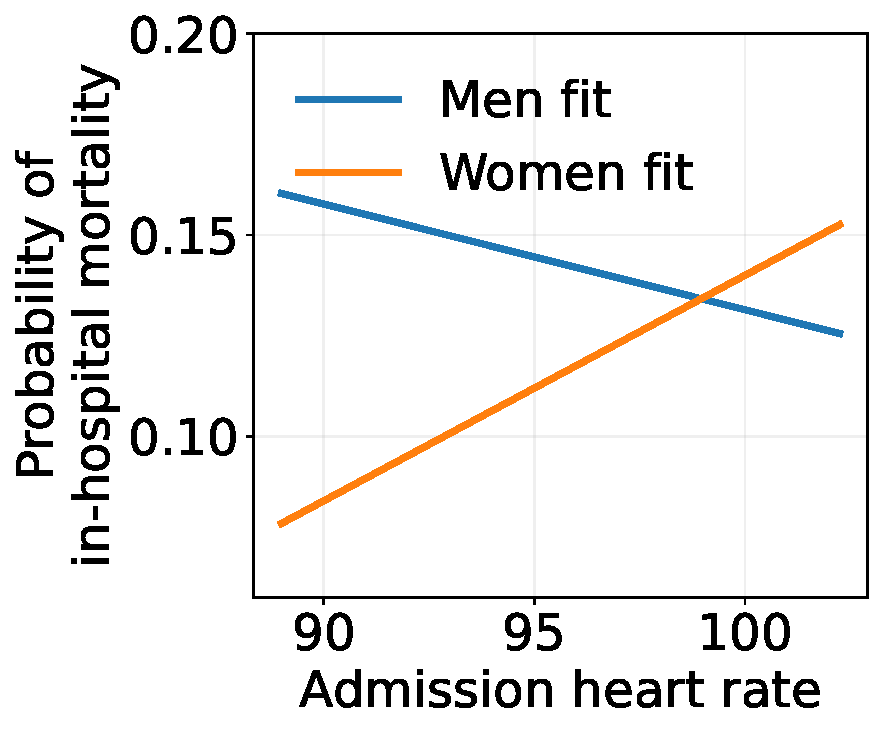
\includegraphics[width=\linewidth]{Sections/Figures/hr_quartile2_mortality_lines.pdf}
        \label{fig:hr_quartile2}
    \end{subfigure}
    %\hfill
    %\begin{subfigure}[t]{0.48\linewidth}
    %    \centering
    %    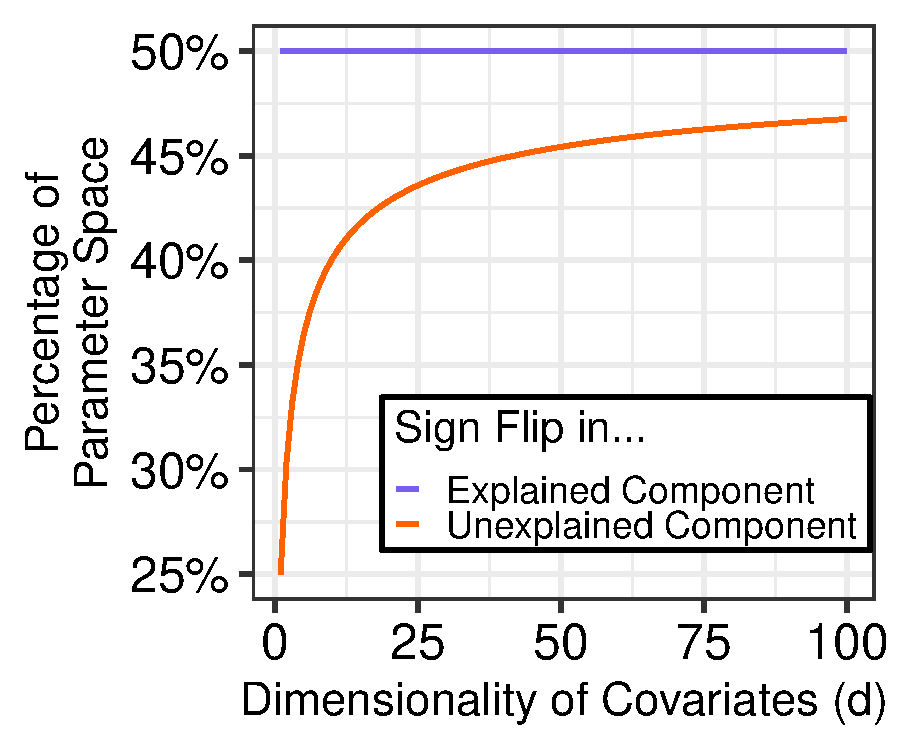
\includegraphics[width=\linewidth]{Sections/Figures/prob_unexplained.pdf}
    %    \label{fig:prob_unexplained}
    %\end{subfigure}
    \caption{Linear fit of mortality on admission heart rate for each group when holding all other covariates fixed at their group means.}
    \label{fig:sign_flip_overview}
\end{figure}


\section{How common are conflicting conclusions?} 
\label{sec:signflips}

Our examples above serve as an existence proof that reference group choice can reverse the OBD's substantive conclusions.
However, a few major questions remain.
First, do these conclusion reversals occur in the absence of finite-sample noise; i.e., do practitioners with large-scale datasets still need to worry about them?
Second, even if conclusion reversals can occur, do they occur outside of mathematically adversarial examples (i.e., ``measure zero'' in some sense)?
Third, when should we expect conflicting conclusions to be more or less frequent?

In this section, we mathematically prove the answer to the first two questions is yes and derive closed-form equations for the probability of conflicting conclusions that allow an intuitive answer to the third question.
\cref{sec:simulated_example} complements our argument with an empirical example where index ambiguity occurs even without sampling noise.

In what follows, we study conclusion reversals that involve the explained or unexplained component changing signs from positive to negative, or vice versa.
To balance mathematical tractability and generality of our theory, we will focus on the OBD under a fairly general class of functions $f^H, f^K$: those drawn from a Gaussian process.
%For mathematical tractability and applicability to practical usage, we continue our focus on the OBD (vs.\ OBD). % (i.e., using linear models in \cref{eq:OB_H_Counterfactual,eq:OB_K_Counterfactual}).
To show that index ambiguity is not an artifact of finite samples, we work in the population limit; since we work in the population limit, statistical significance is no longer a concern.
Put another way, the only decisions available are `positive' or `negative', not `inconclusive.'
And to show that index ambiguity is not a ``measure zero'' phenomenon, we show that conflicting conclusions in general occur with non-zero probability.
% We use our analysis of the parameter space to interpret our empirical exercises and discuss frontier work on the OBD that enriches the covariate space using machine learning models \citep{bach2024heterogeneity,quintero2025,flachaire2025decomposing}.

\subsection{A general computation of index ambiguity probabilities}
\label{sec:general_flip_probabilities}
To answer our three questions, it will be useful to express the frequency of index ambiguity under a given data generating process.
To do so, we treat the functions $f^H$ and $f^K$ as random and the covariate distributions $h$ and $k$ as fixed.
This setup reflects the situations considered throughout our paper, where the populations are fixed (e.g., men and women or Hospital $H$ and Hospital $K$) and potentially well-known to the data scientist, but the response functions are unknown and thus may be considered random.
We let $\nu$ be a distribution over functions $f$ and make the following two assumptions.
%
\begin{assumption} \label{assum:iid}
Assume that $f^K, f^H$ are drawn i.i.d.\ from $\nu$.
\end{assumption}
\begin{assumption} \label{assum:atomless}
	Under \cref{assum:iid}, assume that $\nu$ is such that there is zero probability that any explained or unexplained component is equal to zero.
\end{assumption}
\cref{assum:atomless} is likely satisfied by any continuous distribution $\nu$, and we assume it only to make the resulting probabilities more readable.
Finally, some extra notation will be useful in stating our theoretical results.
\begin{equation}
	V(f) := \int f(x)h(x) dx, \quad W(f) := \int f(x)k(x)dx
\end{equation}
Then the explained component is $V(f^g) - W(f^g)$ for reference group $g$, and the unexplained component with reference group $H$ is $W(f^H) - W(f^K)$, and analogously for reference group $K$.
Now we can prove a basic fact about the probability of index ambiguity.
\begin{proposition} \label{prop:generic_flip_probs}
	Take \cref{assum:atomless,assum:iid}.
	Then the probability of index ambiguity in the explained component is given by
	\begin{equation}
		Pr_\nu(\mathrm{explained\ ambiguity}) = 2 q (1-q), \label{eq:explained_flip_pr}
	\end{equation}
	where $q := \nu(V-W > 0)$.
	For the unexplained component, let $(V,W)$ and $(V', W')$ be i.i.d.\ copies of the pair $(V(f), W(f))$ with $f \sim \nu$. Then:
	\begin{align}
		Pr_\nu(& \mathrm{unexplained\ ambiguity}) \nonumber \\
		& = Pr_\nu \left( (V - V')(W - W') < 0 \right) \label{eq:unexplained_flip_pr}
	\end{align}
\end{proposition}
See \cref{app:proof_generic_flip_probs} for a proof.
\cref{prop:generic_flip_probs} is highly generic, but it is not immediately useful.
In particular, it does not answer the questions of whether conflicting conclusions are adversarial events, and, if not, when we should expect them to occur more or less frequently.
To answer such qualitative questions, we need to compute \cref{eq:explained_flip_pr,eq:unexplained_flip_pr}; we undertake this task in the next section.

\subsection{Index ambiguity probabilities under a GP prior}
\label{sec:gp_sign_flips}
We will specify a particular model for $\nu$ to enable computation of the probabilities in \cref{prop:generic_flip_probs}.
We choose a Gaussian process (GP) for mathematical tractability; however, we note this is not a particularly constraining choice, as the choice of kernel and mean function allows for a rich class of distributions that $f^H$ and $f^K$ might be drawn from.
\begin{assumption} \label{assum:gp}
	$\nu$ is a Gaussian process (GP) with mean function $\mu$ and kernel function $C$. Under this model, define:
	\begin{align*}
		 \langle h, k \rangle_C &:= \int\int C(x,x') h(x) k(x') dx dx' \\
		& \| h \|_C^2 := \langle h, h \rangle_C \quad \| k \|_C^2 := \langle k, k \rangle_C.
	\end{align*}
\end{assumption}
Finally, we will make some regularity assumptions on the kernel and mean function of the GP.
\begin{assumption} \label{assum:fubini}
	The following hold with $m = k$ and $m = h$:
	\begin{equation}
		\int \sqrt{C(x,x)} m(x) dx < \infty, \;\; \int | \mu(x) | m(x) dx < \infty
	\end{equation}
\end{assumption}
These regularity conditions are extremely broad.
E.g., any kernel with $C(x,x)$ equal to a constant (any stationary kernel) satisfies the first, and the second merely states that $\mu$ is integrable with respect to $h$ and $k$.
Under these assumptions, we can derive closed forms for the explained and unexplained index ambiguity.
For notation, we let $\Phi$ be the CDF of the standard normal function.
\begin{proposition} \label{prop:sign_flip_gp}
	Take \cref{assum:iid,assum:atomless,assum:gp,assum:fubini}. Then we have that:
	\begin{align}
		&Pr_\nu[\mathrm{unexplained\ ambiguity}] = \frac{1}{\pi} \arccos\left(\frac{\langle h, k \rangle_C}{\| h \|_C \| k \|_C} \right) \label{eq:unexplained_flip_pr_gp} \\
		&Pr_\nu[\mathrm{explained\ ambiguity}] = 2 \Phi (\lambda) \Phi(-\lambda), \label{eq:explained_flip_pr_gp}
	\end{align}
	where we have used $\lambda := \langle \mu, h-k \rangle / \|h -k\|_C$.
\end{proposition}	
See \cref{app:proof_sign_flip_gp} for a proof.
We can use \cref{prop:sign_flip_gp} to answer our qualitative questions.
First, we can see that the probabilities of index ambiguity are not zero, even in the infinite sample limit where we have exact access to $f^H$ and $f^K$.
Second, we see that for general $h,k, C,\mu$, neither the explained nor unexplained index ambiguity probability is zero; only in highly specific cases such as $h = k$ do we get zero probabilities.
As our model for $\nu$ is fairly generic, we conclude that conflicting conclusions are not an ``adversarial'' or ``measure zero'' phenomenon, and we should expect to encounter them in practice.
Finally, when should we expect index ambiguity to be more or less frequent?
We next consider this question for the explained and unexplained component separately.

\textbf{Explained component.} We see that index ambiguity is likely in the explained component if $| \lambda |$ is small and unlikely if $|\lambda|$ is large.
The numerator of $\lambda$ is large if $h$ and $k$ mainly differ on covariates with large means.
The denominator is small if $h$ and $k$ vary on covariates that, under $C$, have low variance.
Overall, to have a small probability of explained component index ambiguity, it must be that $h$ and $k$ vary primarily on covariates that have a non-zero mean \emph{and} a small variance, i.e., covariates with a high signal-to-noise ratio under $f \sim GP(\mu, C)$.

\textbf{Unexplained component.}
The unexplained index ambiguity probability is driven to zero when $\langle h,k\rangle_C$ is equal to $\| h\|_C \| k \|_C$. 
For intuition about when this will happen, suppose $C$ is a distance-based kernel, like the radial basis function (RBF) kernel. 
Then $\langle h,k\rangle_C$ is large precisely when $h$ puts significant mass in regions of space that are ``close'' to regions of space where $k$ puts significant mass; here, ``close'' is as defined by the length scale of the kernel, and ``large'' is measured with respect to the product $\|h\|_C \|k\|_C$. 
Put differently, if there are many nearby regions of space where $h$ and $k$ are large \emph{and} we expect a randomly drawn $f$ to be relatively constant (because $C$ is high over for pairs of points drawn from across the region), then the probability of unexpected  component index ambiguity is driven down.
Alternatively, if regions where $h$ is high and regions where $k$ is high are sufficiently far apart that we expect $f$ to significantly vary between them, then the probability of an unexplained component index ambiguity is driven up.

%\textcolor{red}{\textbf{Can the explained and unexplained probabilities be simultaneously small?} WTS: putting this here b/c I just think this would be interesting to think and comment on. But we can easily just not put this in the paper.}
\section{Conclusion}
\label{sec:conclusion}

It is well known that the OBD depends on the choice of reference group; however, past work did not establish that the two references could yield conflicting conclusions. 
We here demonstrate that this asymmetry can result in conflicting conclusions between the two reference choices.
We present examples from real datasets as existence proofs. 
We show that sign reversals can occur in either the explained or unexplained component and are not solely products of model misspecification, small sample size, or an adversarial data generating process.

We think it is plausible that many practitioners do not report both references \citep{zhang_2019, ayubiShahbaziKhazaei2024,paradaContzen2025,singleton2016,lamJamiesonMittinty2021,leythienne2021paygapeu,alHanawiNjagi2022,tao2024gender}, and a widely-cited handbook on the OBD does not suggest reporting both references \citep{fortinLemieuxFirpo2011}, because they were not aware that reference choice could be so consequential.
We hope that our work illustrates the importance of reporting both reference groups and convinces practitioners to do so.
%As a practical conclusion, we recommend that data analysts using the OBD always report results using both reference groups to accurately convey the degree of support behind substantive conclusions arising from the OBD.

Our work leaves an important open question: whether there exist alternatives to the OBD that do not suffer from problems of non-robustness to arbitrary choices.
For example, our work has shown that the OBD is not robust to the choice of reference group, and we have noted that the choice of reference group is often arbitrary.
As discussed in \cref{sec:existing_index_number}, there are a number of decomposition methods that do not have the index number problem but require other arbitrary choices.
Future work should examine if any existing decomposition method can reduce or eliminate the non-robustness of the OBD, and, if not, whether any such decomposition method is possible.
If no such robust decomposition exists, then practitioners will be forced to always conduct robustness checks of their results.

%Our theoretical results model only the case where the two populations' response functions are drawn i.i.d.\ from $\nu$.
%Our theoretical results show that the fraction of parameter space representing sign reversals is large for linear models and grows with the dimension of the feature space.
%However, our empirical exercises reveal fewer sign reversals than our theoretical results suggest, implying that fitted linear regression parameters in real data analyses may not be well modeled by a uniform distribution over the parameter space. 
%Future work can determine to what extent our theoretical findings hold for non-uniform parameter distributions, other measures of model complexity, and nonlinear models. 

%\textbf{Broader impacts.}
%The OBD is widely used to draw conclusions and influence policy.
%Our work shows that the choice of reference group in the OBD can reverse substantive conclusions and characterizes conditions under which such reversals can occur.
%We highlight the importance of reporting results for both references, even though this step is currently sometimes omitted in published papers
%and government reports.
%Thus, our work has the potential to improve decisions that arise from using the OBD.
%Our work does have one potential negative societal impact: that researchers learn they may be able to cherry-pick results through the choice of OBD reference group.
%However, a researcher with an agenda can also influence results through sample selection, feature engineering, and model choice; we think it unlikely that reference group choice is the only means to their end.
%If one wishes to cherry-pick, there are already more than enough trees to harvest from, so to speak.
%Further, we suspect (or, hope) that the majority of mis-use of the OBD is from researchers unaware of its problems, and so hope that the net impact from our paper will be positive. 


%Even though it is well-known that the OBD depends on the choice of reference group, we show that this dependence can be highly consequential, leading to sign reversals in both the explained and unexplained components.
%We present real and simulated examples in which such a reversal occurs.%We present a simple healthcare example, inspired by real-world data, as well as a real clinical case study, in which one OBD direction suggests that quality of care improves patient outcomes, while the other suggests it worsens them. 
%We further prove that such sign reversals are not isolated phenomena, but can occur in a wide variety of scenarios. 
%However, we demonstrate that while the set of regression parameters $(\beta_g, \alpha_g, \mu_g), g \in \{K, H\}$ leading to sign flips is substrantial, there is reason to believe sign flips will be rare in practice.
%We therefore believe that practitioners should be cautiously optimistic about use of the OBD: it is likely to provide robust and useful insights about differences between populations, but it is critical that practitioners compute and report its robustness to the choice of reference group, less they be mislead by an arbitrary choice of the reference group.
%Practitioners should therefore be cautious optimistic when using the OBD, at least in settings where no reference group is clearly justified.


\section*{Acknowledgements}
DISTRIBUTION STATEMENT A. Approved for public release. Distribution is unlimited. This material is based upon work supported by the Combatant Commands under Air Force Contract No. FA8702-15-D-0001 or FA8702-25-D-B002. Any opinions, findings, conclusions or recommendations expressed in this material are those of the author(s) and do not necessarily reflect the views of the Combatant Commands.

\bibliographystyle{icml2026}
\bibliography{OBD_signflip}

%%%%%%%%%%%%%%%%%%%%%%%%%%%%%%%%%%%%%%%%%%%%%%%%%%%%%%%%%%%%
\clearpage
\appendix
\section{Extended literature review}
\label{appendix:lit_review_xAI}

In this appendix, we expand on the discussion in \cref{sec:intro} of why standard explainability methods do not address the hospital data scientist's question from \cref{sec:intro}, and of how the OBD differs from these methods.
We then discuss how common modifications to the OBD that might seem to remove the index number problem either do not or introduce new questions of arbitrariness similar to the index number problem.

\subsection{Explainability methods for attributing outcome behavior to covariates}
\label{appendix:xAI}

A common feature of modern explainability methods, including Shapley values \citep{Shapley1953, Lundberg2017, chen2025shapley}, Functional ANOVA \citep{stone1994, hooker2004discovering, hookerGeneralizedFunctionalANOVA2007, lengerich2020purifying, fumagalli2025fanova}, Accumulated Local Effects \citep{apley2020}, and partial dependence plots \citep{friedman2001greedy, liu2025trees}, is that they take as their input a fitted outcome model, or more generally a conditional mean function $x \mapsto \E[Y \mid X=x]$.
They ask how this function changes as one or more covariates change, or how much variation in the function can be attributed to particular (groups of) covariates.
This type of decomposition is well-suited to many tasks in machine learning explainability, but does not, by itself, separate differences between two populations into differences in the distribution of $X$ versus differences in the distribution of $Y \mid X$.
We elaborate on this distinction below for three common decomposition methods.

Functional ANOVA measures the importance of features in determining the output of a function $f$ and identifies underlying additive interactions between subsets of covariates \citep{hooker2004discovering, hookerGeneralizedFunctionalANOVA2007}.
It represents $f$ as a sum of an overall mean, main effects of individual covariates, pairwise interactions, tertiary interactions, etc. The definitions of these terms depends on a reference measure over the covariates that pins down the orthogonality and centering (mean zero) restrictions.
Accumulated Local Effects \citep[ALE;][]{apley2020} and partial dependence plots \citep[PDP;][]{friedman2001greedy} summarize how a fitted function changes with one covariate or a subset of covariates; for instance, how predicted mortality varies with admission heart rate, but they do not define a decomposition of the gap between two groups and at least it is not clear how to use them to do so; one can similarly define an additive decomposition of a function $f$ using PDP or ALE.
But Functional ANOVA, ALE, and PDP are tools for decomposing a \emph{single} function $f$, not for studying differences between two functions, which is the problem addressed by the OBD.
We are aware of only one work applying ALE and Functional ANOVA to generalize the OBD \citep{quintero2025}; however, \citet{quintero2025} shows this leads to serious issues beyond just the index number problem studied here.
% But the role this single reference measure plays in Functional ANOVA is not the role played by the covariate distribution in the OBD.
% Functional ANOVA uses one reference measure to decompose one function $f$, whereas the OBD uses two distinct covariate distributions and two distinct conditional means to attribute the gap $\E_H[Y] - \E_K[Y]$ to changes in $X$ versus changes in $Y \mid X$.
% Applying Functional ANOVA separately to $f_H(x) = \E_H[Y \mid X=x]$ and $f_K(x) = \E_K[Y \mid X=x]$ would yield two decompositions of two functions, not the counterfactual means $\E_K[f_H(X)]$ and $\E_H[f_K(X)]$ needed to separate differences in $X$ from differences in $Y \mid X$.

% Accumulated Local Effects \citep[ALE;][]{apley2020} and partial dependence plots \citep[PDP;][]{friedman2001greedy} summarize how a fitted function changes with one covariate or a subset of covariates; for instance, how predicted mortality varies with admission heart rate, but they do not define a decomposition of the gap between two groups and at least it is not clear how to use them to do so.
% An ALE curve or partial dependence plot for $f_H$ cannot say what Hospital $H$'s mortality rate would be if its patients had the risk factor distribution of Hospital $K$, and the corresponding curve for $f_K$ cannot answer the reverse counterfactual.

Shapley-value-based methods are feature attribution tools that assign each covariate a portion of a prediction, or of the variation in predictions, by treating the covariates as players in a cooperative game whose payoff is the model's output \citep{Shapley1953, Lundberg2017, chen2025shapley}.
Again, though, Shapley values are useful for attributing the output of a single fitted model to features, not a situation in which there are two populations.
In \cref{sec:existing_index_number} we detail one way in which Shapley values could be used to produce a decomposition for differences between populations like the one produced by the OBD, and this decomposition does not have an index number problem. However, we discuss in \cref{sec:existing_index_number} why such a possible solution actually introduces other issues.

\subsection{Adaptations of the Oaxaca--Blinder decomposition beyond linear models}
\label{appendix:obd_generalized}

% The OBD addresses precisely the shortcoming above by comparing observed means to counterfactual means of the form $\E_{g'}[\E_g[Y \mid X]]$, where the conditional distribution $Y \mid X$ is taken from one group and the covariate distribution from the other; see \cref{eq:OB_H_Counterfactual,eq:OB_K_Counterfactual} in \cref{sec:counterfactual_OBD}.
The OBD was developed for linear models \citep{oaxaca1973, blinder1973} and remains widely used in this form across applied health, labor, and policy research \citep{paradaContzen2025, barhaim2023, cartwright2021}.
Still, recent work has paired the OBD with flexible ML estimators to relax the linearity assumption while retaining the between-population counterfactual structure of \cref{eq:OB_H_Counterfactual,eq:OB_K_Counterfactual}.
We review these efforts here.
\citet{bach2024heterogeneity} use double-lasso to fit a high-dimensional wage equation and quantify how the US wage gap between men and women varies with characteristics such as marital status, race, occupation, and education.
\citet{mao2025double} apply the double machine learning framework to the Oaxaca--Blinder decomposition, deriving $\sqrt{n}$-consistent estimators of the composition (i.e., explained) and structure (i.e., unexplained) effects under high-dimensional mixed covariates via Neyman orthogonal scores.
\citet{quintas2024multiply} introduce a multiply-robust estimator for causal change attribution that combines regression and reweighting, remains consistent under partial misspecification of the nuisance ML models, and is asymptotically normal.
\citet{flachaire2025decomposing} reformulate the decomposition in terms of potential outcomes and pair the weighted reference outcome of \citet{neumark1988} with double machine learning to avoid the common-support and trimming requirements that arise when the reference is taken to be one of the two groups.
Closer to our setting, \citet{quintero2025} examine what happens when off-the-shelf functional decompositions, specifically Functional ANOVA and ALE, are plugged into the OBD framework, and show that they can misattribute differences in $X$ to differences in $Y \mid X$.

In all of these methods, $\E_H[Y \mid X]$ and $\E_K[Y \mid X]$ are estimated by flexible $\hat{M}_H(X)$ and $\hat{M}_K(X)$, and counterfactual means are constructed as in \cref{eq:OBD_H_estimated}.
Such methods retain the between-population target of the OBD and so address the limitation of the explainability methods above.
However, with the exception of \citet{flachaire2025decomposing}, who fix a single Neumark-style weighted reference \citep{neumark1988}, this line of work does not engage with the issue we study.
That is, even once linearity is relaxed, the OBD still requires choosing one of the two groups as a reference, and this choice can affect the numerical result; more importantly, as we show, it can reverse substantive conclusions.
%Even if the conditional mean functions were estimated without error, the explained components $E^{(H)}$ and $E^{(K)}$ (and analogously $U^{(H)}$ and $U^{(K)}$) need not have the same sign.
Improving the flexibility of $\hat{M}_g$ thus does not remove the index number problem; if anything, richer models may make the issue worse, as \cref{tab:flip_summary_main} shows for our main empirical exercise.

In short, adaptations of the OBD and explainability methods address different parts of the overall problem: explainability methods describe how a single fitted function depends on covariates, while the OBD improves the estimation of the conditional mean functions used to form counterfactual means.
Our paper studies distinct questions --- whether the two natural OBD references can yield substantively different conclusions, and how common this sensitivity is.

\subsection{Existing solutions to the index number problem}
\label{sec:existing_index_number}
A few proposed methods exist that compute decompositions similar to the OBD, and yet do not have the index number problem.
We describe the approach of these options here and discuss how they do not resolve the issue of arbitrariness discussed in this paper.

\textbf{Shapley Values.} Shapley values \citep{Shapley1953} are widely used in the machine learning literature to understand a models' predictions.
A straightforward use of them would be to estimate ``explained'' or ``unexplained'' contributions to $\Delta_Y$.
This follows from the standard Shapley construction, which treats each reference-based decomposition as a ``player'' and assigns contributions by averaging marginal effects over all orderings; with two ``players'' (the two reference directions $H$ and $K$), there are two equally weighted permutations, $(H,K)$ and $(K,H)$, so the Shapley value reduces to the simple average, for the explained component, $E = \tfrac{1}{2}E^{(H)} + \tfrac{1}{2}E^{(K)}$.

However, our paper complicates the interpretation of $E^{(H)}$ and $E^{(K)}$ (and likewise for the unexplained components). 
If the explained component can take on opposite signs depending on the reference group, it is ambiguous whether the distributions of covariates widen or shrink the gap in outcomes between $H$ and $K$.
It is not clear that averaging across the reference groups appropriately resolves this ambiguity; for instance, if $E^{(H)}$ and $E^{(K)}$ can take opposite signs, averaging them destroys information about their magnitude.
For example, $\tfrac{1}{2}E^{(H)} + \tfrac{1}{2}E^{(K)}$ can take on small positive values if $E^{(H)}$ and $E^{(K)}$ are both small and positive, or both large but and of opposing signs. 
A researcher may wish to distinguish between these scenarios, but the Shapley proposal above does not.

\textbf{Pooled approaches.}
Another approach to eliminate the index number problem is to define some ``pooled'' group and then measure deviations from this group in a three-term decomposition. For example, in the case of the (linear) OBD, one defines a pooled $\beta^*$ and then computes:
% two-column layout: split over two lines (no symbols changed). Original kept below.

\begin{align}
  \E_H[Y] - \E_K[Y] &= (\mu_H - \mu_K)^T \beta^* \nonumber \\
  &\quad + \mu_H^T (\beta_H - \beta^*) + \mu_K^T(\beta^* - \beta_K).
\end{align}
%REV \begin{equation}
%REV   \E_H[Y] - \E_K[Y] = (\mu_H - \mu_K)^T \beta^* + \mu_H^T (\beta_H - \beta^*) + \mu_K^T(\beta^* - \beta_K).
%REV \end{equation}
The first term is interpreted as differences due differences in covariates, the second differences due to differences in $H$'s $Y \mid X$ from the baseline, and the third differences due to differences in $K$'s $Y \mid X$ from the baseline.

The question that remains, then is how to define $\beta^*$.
A typical choice is to use some sort of ``average'' of the two groups.
One approach from \citet{oaxacaRansom1998}, defines some $w \in [0,1]$ and sets $\beta^* = (1-w)\beta_K + w\beta_H$.
A second approach, from \citet{neumark1988}, is to create a pooled dataset consisting of all samples from $H$ and $K$, and estimate $\beta^*$ from this dataset.
However, these approaches suffer from issues of arbitrariness as well.
First, how does one pick $w$ in the Oaxaca-Ransom approach?
Second, why is defining $\beta^*$ one way more reasonable than the other?
If we assume both are equally reasonable, then, given our results for the OBD, we feel that one should be highly suspicious of substantive conclusions being robust to the choice of $\beta^*$.
Finally, justifications for a choice of $w$ or $\beta^*$ in one research setting may not apply in others.
For example, in analyses of the labor market, $\beta^*$ is sometimes intended to represent the $Y \mid X$ relationship in the absence of wage discrimination \citep{neumark1988}. 
There may be no corresponding concept to serve as a reference point in other research contexts; or, there may be no feasible approach for estimating such a reference point.

\textbf{Intermediate covariate distributions.}
\citet{dinardoFortinLemieux1996} propose a variant of the OBD with a more fine-grained decomposition of the explained component, and \citet{quintero2025} propose a OBD with a similarly fine-grained explained decomposition (\citet{quintero2025} also decomposes the unexplained component).
Both cases define a number of intermediate distributions over covariates $P_1, \dots, P_I$, where $P_1 = K_X$ and $P_I = H_X$. E.g., in the case of \citet{quintero2025}, $P_2$ is equal to $K$, except that the marginal of the first covariate is equal to the marginal of $H_X$.
In either case, for each $i = 2, \dots, I$, intermediate explained components are defined as one of:
\begin{align}
  \E_{X \sim P_i}[ \E_{Y \sim H}[Y \mid X] ] - \E_{X \sim P_{i-1}} [ \E_{Y \sim H} [Y \mid X]] \\
  \E_{X \sim P_i}[ \E_{Y \sim K}[Y \mid X] ] - \E_{X \sim P_{i-1}} [ \E_{Y \sim K} [Y \mid X]].
\end{align}  
There are two issues with such approaches.
First, \citet{dinardoFortinLemieux1996} does not change how the the unexplained component is computed over the OBD, so the same exact index number problems with the unexplained component detailed here apply to the decomposition of \citet{dinardoFortinLemieux1996}.
Second, one now has to justify not just a choice of $H$ or $K$ as a reference group, but instead a whole ordering of the $P_i$.
This problem is explicitly called out by \citet{quintero2025}, who choose to fix an arbitrary order.
Given our results here, we suspect that conclusions may not be robust to the ordering of the $P_i$, and we leave such investigation for future work.

\section{Details on Real-Data Examples}
\subsection{ICU Mortality Example}
\label{appendix:icu_details}

This appendix provides full details on how we constructed the ICU data subsets, prepared the analytic dataset, estimated the OBD, identified sign reversals, and computed bootstrap standard errors for all data subsets used in \cref{sec:real_example}. The analyses use the PhysioNet ICU cohort collected for the study of in-hospital mortality \citep{goldberger2000physiobank,silva2012predicting,pollard_physionet_2026}. The raw cohort contains routine admission measurements for $3,997$ patients with known sex ($2,246$ women and $1,751$ men). We merge these records with the corresponding mortality outcomes and restrict attention to patients with complete information on the covariates used in the decomposition: age, ICU type, heart rate (HR), mean arterial pressure (MAP), temperature, urine output, and the indicator for in-hospital death. After removing observations with missing covariates, the final analytic dataset contains $3,429$ patients. All data subset definitions, model specifications, and statistical procedures described below are applied to this cleaned dataset.

\subsection*{Model specification}

For each data subset, we fit separate group-specific models of in-hospital mortality for men and for women. Let $g \in \{\text{men}, \text{women}\}$, let $Y$ be the indicator for in-hospital mortality, and let $X$ be the vector of admission covariates (heart rate, mean arterial pressure, temperature, urine output, age, and ICU type). For each group $g$, we fit an estimator $\hat{f}^g(X)$ of the conditional expectation $\E[Y \mid X, g]$ and use \cref{eq:OB_H_Counterfactual,eq:OB_K_Counterfactual}; see \cref{sec:ob_real}. We consider five model classes, specified as follows.

\textbf{Linear regression.} We take
\[
    \E[Y \mid X, g] \;=\; \alpha_{g} + X^{\top}\beta_{g},
\]
with the group-specific intercept $\alpha_{g}$ and slope $\beta_{g}$ estimated by ordinary least squares. Although $Y$ is binary, this linear probability model is the object to which the classical OBD applies and remains standard in applied work \citep{jann2008, edokaChangesCatastrophicHealth2017, sujin_LPM_OB, mweembaGapSelfRatedHealth2023}.

\textbf{Logistic regression.} Within each group, we standardize the covariates to zero mean and unit variance and fit a logistic regression of $Y$ on the standardized covariates with the default $L_2$ penalty.

\textbf{Neural network.} Within each group, we standardize the covariates and fit a two-hidden-layer fully-connected ReLU network with hidden widths $(32, 16)$, $L_2$ weight decay $10^{-4}$, the Adam optimizer \citep{kingma2015adam}, and max\_iter $=2000$.

\textbf{XGBoost.} We fit a gradient-boosted tree classifier with $250$ estimators, maximum depth $3$, learning rate $0.05$, row subsampling rate $0.9$, column subsampling rate $0.9$, $L_2$ leaf regularization $\lambda = 1.0$, histogram tree method, and the logistic (log-loss) objective.

\textbf{TabPFN.} We use a modern transformer-based tabular model, TabPFN \citep{hollmann2023tabpfn}\footnote{TabPFN uses a custom license: \url{https://huggingface.co/Prior-Labs/tabpfn_2_6/blob/main/LICENSE}}, a pre-trained in-context classifier that maps a training set directly to a predictive distribution for $Y \mid X$. We use the publicly released v2.6 weights and use the v7.1.1 TabPFN code for inference. We run the model locally on a single NVIDIA A100 GPU with $80$~GB of vRAM.

For all five models, we take the predicted probability of in-hospital death as $\hat{f}^g(X)$ and estimate each OBD counterfactual mean $\E_{g'}[\E_g[Y \mid X]]$ by the within-sample average $\frac{1}{|g'|}\sum_{i \in g'} \hat{f}^g(X_i)$.

\subsection*{Data subset construction}
The goal of this analysis was not to target any particular physiological pattern, but rather to explore systematically whether sign reversals arise in realistic data partitions that a practitioner might naturally encounter.

We constructed $139$ data subsets in total. These sets include: quartiles of each continuous admission vital (heart rate, MAP, temperature, urine output);
deciles of age; ICU-type specific cohorts; clinically motivated threshold subsets (HR $>100$, MAP $<65$, Temp $> 38^\circ$C, Urine $>1000$ mL); fifty random $50\%$ subsamples of the cohort; fifty random $30\%$ subsamples of the cohort.

For each data subset and each of the five models in our model class, we compute the decomposition under both reference groups, taking men and women in turn. We say that the explained or unexplained component sign flips in that data subset if its estimated value has opposite signs under the two reference choices. To assess whether such flips are robust to sampling variability, we next describe the bootstrap procedure we use to compute standard errors and $p$-values for each component.

\textbf{Bootstrap.}
For each data subset and each model, we compute bootstrap standard errors and $p$-values for the OBD components. The bootstrap procedure follows the standard Oaxaca--Blinder framework: men and women are resampled within group with replacement, preserving group sizes. For each bootstrap replication $b=1,\dots,B$, we re-fit the corresponding group-specific model and re-estimate the OBD components.

Let $\hat\theta$ denote any Oaxaca--Blinder component (for example, the explained component under the women reference model), and let $\hat\theta^{(1)},\dots,\hat\theta^{(B)}$ denote its bootstrap replicates. The bootstrap standard error and mean are
\[
    \widehat{\operatorname{se}}(\hat\theta)
    =
    \sqrt{
    \frac{1}{B-1}\sum_{b=1}^B
    \bigl(\hat\theta^{(b)} - \bar\theta\bigr)^2
    },
    \qquad
    \bar\theta = \frac{1}{B}\sum_{b=1}^B \hat\theta^{(b)}.
\]
$P$-values are computed using a normal approximation,
\[
    p = 2\left(1 - \Phi\left(\frac{|\hat\theta|}{\widehat{\operatorname{se}}(\hat\theta)}\right)\right).
\]

We say that a sign flip is significant at level $\alpha$ if, in addition to having opposite signs across reference groups, at least one of the two reference-specific estimates has $p < \alpha$. We summarize the total number of data subsets exhibiting any sign flip under each model in \cref{tab:flip_summary_main} in \cref{sec:real_example}. Here, \cref{tab:flip_summary_explained,tab:flip_summary_unexplained} below report the same counts separately for the explained and unexplained components.

We observed that empirically, the count of data subsets exhibiting a sign flip grows with model complexity for this particular data analysis. With the linear and logistic models showing the least amount of sign flips and only a couple remain significant at conventional thresholds. While the neural network and XGBoost show a substantial fraction of data subsets exhibits significant flips even at the $5\%$ level. Importantly, many of the flipped data subsets arise within the random subsamples, indicating that the OBD can yield unstable conclusions even when applied to simple resampled partitions of the same population. Several physiologically interpretable groups also displayed sign changes. The HR quartile two data subset examined in \cref{sec:real_example} is one such case, and serves as a concrete illustration of how these reversals can appear in clinically meaningful settings.

\begin{table}[!ht]
    \caption{Number of data subsets (out of $139$) exhibiting a sign flip in the explained component, by model. Columns $10\%$, $5\%$, and $1\%$ report the number of flipped data subsets that are significant at the corresponding level.}
    \label{tab:flip_summary_explained}
    \centering
    \small
    \begin{tabular}{lcccc}
    \toprule
    Model & Total flips & $10\%$ & $5\%$ & $1\%$ \\
    \midrule
    Linear      & 11 &  2 &  2 &  2 \\
    Logistic    &  9 &  2 &  2 &  1 \\
    Neural net  & 42 & 26 & 17 &  6 \\
    XGBoost     & 33 & 17 & 10 & 3 \\
    TabPFN      & 33 & 21 & 19 & 5 \\
    \bottomrule
    \end{tabular}
\end{table}

\begin{table}[!ht]
    \caption{Number of data subsets (out of $139$) exhibiting a sign flip in the unexplained component, by model. Columns $10\%$, $5\%$, and $1\%$ report the number of flipped data subsets that are significant at the corresponding level.}
    \label{tab:flip_summary_unexplained}
    \centering
    \small
    \begin{tabular}{lcccc}
    \toprule
    Model & Total flips & $10\%$ & $5\%$ & $1\%$ \\
    \midrule
    Linear      & 17 &  0 &  0 &  0 \\
    Logistic    & 21 &  0 &  0 &  0 \\
    Neural net  & 49 & 10 &  6 &  1 \\
    XGBoost     & 47 & 3 &  1 &  0 \\
    TabPFN      & 56 & 2 &  0 &  0 \\
    \bottomrule
    \end{tabular}
\end{table}

A substantial number of these sign reversals are significant at conventional thresholds, indicating that the instability documented in \cref{sec:real_example} is an inherent behavior of the OBD in this clinical dataset.


% \begin{table}[!t]
%     \centering
%     \caption{ICU Mortality Gap Decomposition for Data Subsets Exhibiting Sign Reversals. Standard errors in parentheses computed via bootstrap resampling with $1{,}000$ replications.  
%     P-values based on a normal approximation.  
%     Significance levels: * $p<0.10$, ** $p<0.05$, *** $p<0.01$.  
%     The decomposition separates the gender mortality gap (male minus female) into explained and unexplained components using the Oaxaca--Blinder method.  
%     Female Reference uses the model for females as the reference outcome structure; Male Reference uses the model for males.}
%     \label{tab:icu_mortality}
%     \scriptsize
%     \begin{tabular}{@{}lc*{5}{c}@{}}
%     \toprule
%     \multirow{2}{*}{Subset} &
%     \multirow{2}{*}{n} &
%     Gap &
%     \multicolumn{2}{c}{Female Reference} &
%     \multicolumn{2}{c}{Male Reference} \\
%     \cmidrule(lr){3-3} \cmidrule(lr){4-5} \cmidrule(lr){6-7}
%     & & (M–F) & Expl. & Unexp. & Expl. & Unexp. \\
%     \midrule
    
%     Age decile 1 & 344 & 0.027 & 0.002 & 0.025 & 0.036$^{*}$ & $-0.009$ \\
%     & & (0.033) & (0.009) & (0.033) & (0.019) & (0.030) \\[0.3em]
    
%     Age decile 2 & 347 & 0.004 & 0.023 & $-0.019$ & $-0.010$ & 0.015 \\
%     & & (0.033) & (0.021) & (0.041) & (0.014) & (0.036) \\[0.3em]
    
%     Age decile 4 & 372 & $-0.015$ & 0.012 & $-0.027$ & $-0.004$ & $-0.012$ \\
%     & & (0.032) & (0.013) & (0.035) & (0.017) & (0.037) \\[0.3em]
    
%     Age decile 5 & 344 & $-0.025$ & 0.010 & $-0.035$ & $-0.008$ & $-0.017$ \\
%     & & (0.039) & (0.016) & (0.039) & (0.022) & (0.042) \\[0.3em]
    
%     Age decile 9 & 325 & $-0.077$ & 0.001 & $-0.078$ & 0.001 & $-0.078$ \\
%     & & (0.048) & (0.023) & (0.049) & (0.013) & (0.049) \\[0.3em]
    
%     \textbf{HR quartile 2} & 816 & 0.035 & 0.021$^{***}$ & 0.014 & $-0.007$ & 0.042$^{*}$ \\
%     & & (0.023) & (0.007) & (0.025) & (0.011) & (0.025) \\[0.3em]
    
%     MAP quartile 0 & 877 & $-0.014$ & $-0.003$ & $-0.011$ & 0.004 & $-0.018$ \\
%     & & (0.026) & (0.009) & (0.026) & (0.008) & (0.026) \\[0.3em]
    
%     MAP quartile 1 & 840 & 0.024 & 0.036$^{***}$ & $-0.012$ & 0.011 & 0.013 \\
%     & & (0.022) & (0.012) & (0.027) & (0.008) & (0.022) \\[0.3em]
    
%     Urine quartile 0 & 859 & $-0.031$ & 0.007 & $-0.038$ & $-0.006$ & $-0.025$ \\
%     & & (0.027) & (0.009) & (0.027) & (0.007) & (0.027) \\[0.3em]
    
%     MAP $< 65$ & 697 & $-0.028$ & $-0.011$ & $-0.017$ & 0.002 & $-0.030$ \\
%     & & (0.029) & (0.012) & (0.029) & (0.008) & (0.029) \\[0.3em]
    
%     Temp $> 36.5$ & 267 & $-0.043$ & $-0.001$ & $-0.042$ & 0.008 & $-0.051$ \\
%     & & (0.047) & (0.025) & (0.050) & (0.019) & (0.046) \\[0.3em]
    
%     Urine $> 1000$ & 210 & 0.046 & $-0.014$ & 0.060 & 0.014 & 0.031 \\
%     & & (0.036) & (0.018) & (0.038) & (0.023) & (0.037) \\[0.3em]
    
%     Random 50\% \#6 & 1714 & 0.020 & 0.023$^{***}$ & $-0.003$ & 0.012$^{**}$ & 0.009 \\
%     & & (0.017) & (0.005) & (0.018) & (0.006) & (0.017) \\[0.3em]

%     Random 50\% \#21 & 1714 & 0.018 & 0.019$^{***}$ & $-0.001$ & 0.015$^{***}$ & 0.003 \\
%     & & (0.016) & (0.005) & (0.017) & (0.005) & (0.015) \\[0.3em]

%     Random 50\% \#28 & 1714 & 0.013 & 0.016$^{***}$ & $-0.004$ & 0.009$^{**}$ & 0.003 \\
%     & & (0.018) & (0.005) & (0.018) & (0.004) & (0.017) \\[0.3em]

%     Random 50\% \#30 & 1714 & 0.008 & 0.014$^{***}$ & $-0.006$ & 0.004 & 0.005 \\
%     & & (0.017) & (0.005) & (0.018) & (0.004) & (0.017) \\[0.3em]

%     Random 50\% \#34 & 1714 & 0.009 & 0.016$^{***}$ & $-0.007$ & 0.009$^{*}$ & 0.001 \\
%     & & (0.015) & (0.005) & (0.016) & (0.005) & (0.015) \\[0.3em]

%     Random 50\% \#39 & 1714 & 0.019 & 0.020$^{***}$ & $-0.001$ & 0.012$^{**}$ & 0.007 \\
%     & & (0.017) & (0.005) & (0.018) & (0.005) & (0.016) \\[0.3em]

%     Random 30\% \#0 & 1028 & 0.018 & 0.018$^{***}$ & $-0.001$ & 0.008 & 0.010 \\
%     & & (0.022) & (0.006) & (0.023) & (0.006) & (0.021) \\[0.3em]

%     Random 30\% \#5 & 1028 & 0.011 & 0.016$^{***}$ & $-0.005$ & 0.008 & 0.003 \\
%     & & (0.020) & (0.006) & (0.021) & (0.008) & (0.021) \\[0.3em]

%     Random 30\% \#17 & 1028 & 0.008 & 0.014$^{**}$ & $-0.006$ & 0.008 & 0.000 \\
%     & & (0.022) & (0.007) & (0.023) & (0.006) & (0.022) \\[0.3em]

%     Random 30\% \#18 & 1028 & 0.007 & 0.022$^{***}$ & $-0.015$ & 0.002 & 0.004 \\
%     & & (0.022) & (0.007) & (0.024) & (0.005) & (0.022) \\[0.3em]

%     Random 30\% \#20 & 1028 & 0.002 & 0.001 & 0.001 & 0.005 & $-0.003$ \\
%     & & (0.020) & (0.007) & (0.020) & (0.005) & (0.019) \\[0.3em]

%     Random 30\% \#24 & 1028 & 0.021 & 0.018$^{***}$ & 0.003 & $-0.007$ & 0.027 \\
%     & & (0.021) & (0.007) & (0.023) & (0.010) & (0.023) \\[0.3em]

%     Random 30\% \#31 & 1028 & 0.015 & 0.014$^{**}$ & 0.000 & 0.023$^{***}$ & $-0.009$ \\
%     & & (0.021) & (0.007) & (0.022) & (0.009) & (0.020) \\[0.3em]

%     Random 30\% \#37 & 1028 & 0.011 & 0.021$^{**}$ & $-0.011$ & 0.007 & 0.004 \\
%     & & (0.023) & (0.009) & (0.025) & (0.006) & (0.022) \\[0.3em]

%     Random 30\% \#43 & 1028 & 0.015 & 0.017$^{**}$ & $-0.002$ & 0.012$^{**}$ & 0.003 \\
%     & & (0.021) & (0.007) & (0.023) & (0.006) & (0.021) \\
    
%     \bottomrule
%     \end{tabular}
% \end{table}
    
\subsection*{HR quartile 2: results across models}
\label{appendix:hrq2}

\cref{sec:real_example} focuses on the HR quartile two data subset under the OBD. In \cref{tab:hrq2_bootstrap_models}, we report the corresponding decomposition under each of the five models in our model class. The linear, logistic, neural-network, and XGBoost results are obtained from the bootstrap procedure described above with $B = 1{,}000$ replications.

% table* because the appendix is set in two columns (layout only).
\begin{table*}[!ht]
    \caption{OBD of the sex mortality gap in HR quartile two ($n = 816$), across all five models. The total gap is men's mean minus women's mean. Standard errors in parentheses are computed via bootstrap resampling with $1{,}000$ replications. $p$-values are based on a normal approximation (Wald test). Significance levels: * $p<0.10$, ** $p<0.05$, *** $p<0.01$.}
    \label{tab:hrq2_bootstrap_models}
    \centering
    \scriptsize
    \begin{tabular}{@{}lc*{4}{c}@{}}
    \toprule
    \multirow{2}{*}{Model} &
    \multirow{2}{*}{Gap (M--F)} &
    \multicolumn{2}{c}{Women reference} &
    \multicolumn{2}{c}{Men reference} \\
    \cmidrule(lr){3-4} \cmidrule(lr){5-6}
    & & Explained & Unexplained & Explained & Unexplained \\
    \midrule

    Linear
        & \makecell{$0.035$ \\ $(0.023)$}
        & \makecell{$0.021^{***}$ \\ $(0.007)$}
        & \makecell{$0.014$ \\ $(0.025)$}
        & \makecell{$-0.007$ \\ $(0.010)$}
        & \makecell{$0.042^{*}$ \\ $(0.025)$} \\[0.3em]

    Logistic
        & \makecell{$0.035$ \\ $(0.023)$}
        & \makecell{$0.026^{***}$ \\ $(0.009)$}
        & \makecell{$0.009$ \\ $(0.025)$}
        & \makecell{$-0.006$ \\ $(0.008)$}
        & \makecell{$0.041^{*}$ \\ $(0.024)$} \\[0.3em]

    Neural net
        & \makecell{$0.035$ \\ $(0.023)$}
        & \makecell{$0.001$ \\ $(0.024)$}
        & \makecell{$0.033$ \\ $(0.031)$}
        & \makecell{$0.053^{**}$ \\ $(0.022)$}
        & \makecell{$-0.018$ \\ $(0.025)$} \\[0.3em]

    XGBoost
        & \makecell{$0.035$ \\ $(0.023)$}
        & \makecell{$0.004$ \\ $(0.016)$}
        & \makecell{$0.031$ \\ $(0.025)$}
        & \makecell{$0.029^{**}$ \\ $(0.014)$}
        & \makecell{$0.006$ \\ $(0.021)$} \\[0.3em]

    TabPFN
        & \makecell{$0.035$ \\ $(0.023)$}
        & \makecell{$0.012$ \\ $(0.016$}                                                                                                                                                                                                                                                                              
        & \makecell{$0.023$ \\ $(0.026)$}
        & \makecell{$0.023^{*}$ \\ $(0.013)$} 
        & \makecell{$0.012$ \\ $(0.021)$} \\[0.3em]
    \bottomrule
    \end{tabular}
\end{table*}

The linear and logistic OBD exhibit a consistent explained-component sign flip that is significant at the $1\%$ level, with very similar magnitudes: in both cases, the explained component is significantly positive under the women reference and flips to a small negative (non-significant) value under the men reference. The neural network and XGBoost both point to the men reference estimate being significantly positive at the $5\%$ level.

\cref{fig:hr_quartile2_hist} presents the histogram for the $816$ patients in HR quartile two, showing the distribution of mortality outcomes used in the linear probability models displayed in \cref{fig:sign_flip_overview} (left). \cref{tab:delta_mu_betas} shows the covariate mean differences and group-specific coefficients for HR quartile two that underlie the sign reversal documented in \cref{sec:real_example}.

\begin{figure}[!ht]
        \centerline{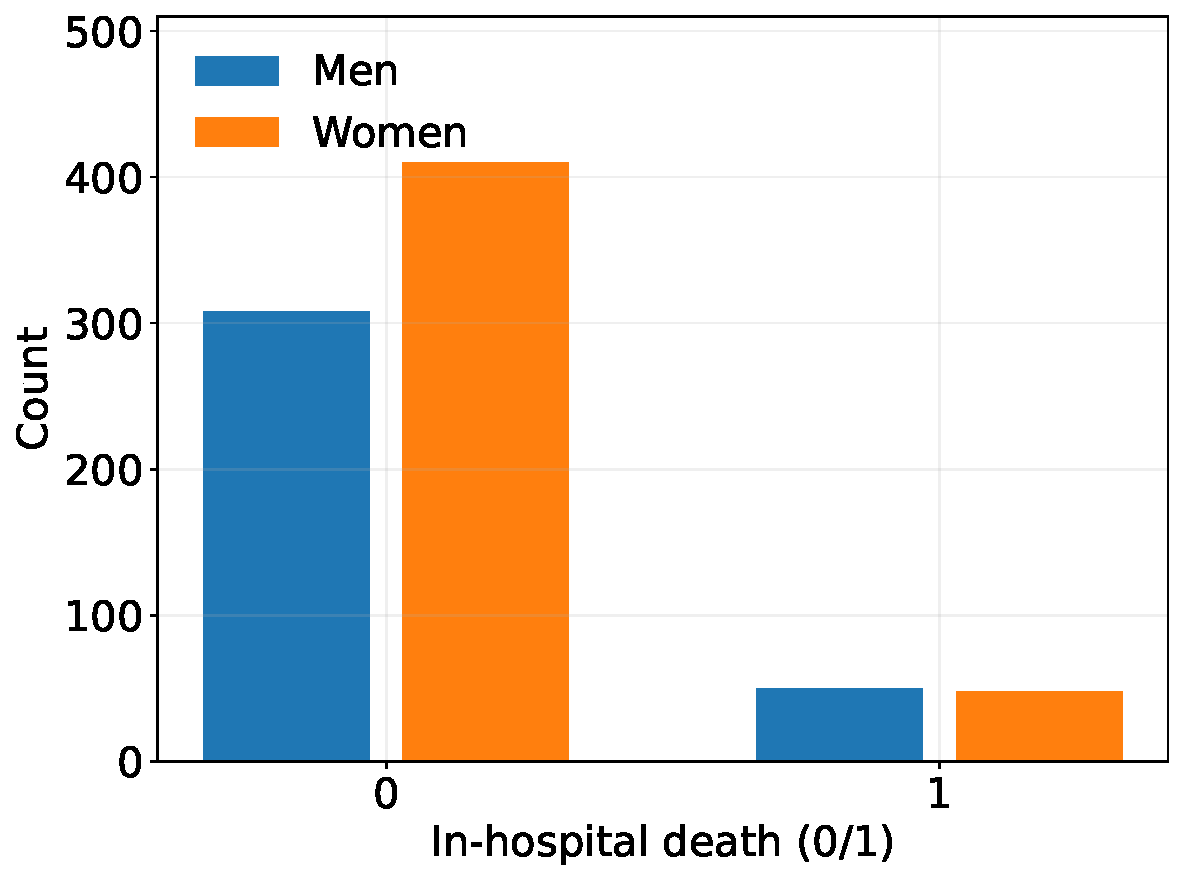
\includegraphics[width=0.42\linewidth]{Sections/Figures/hr_quartile2_mortality_y_hist.pdf}}
    \caption{Mortality outcome histogram for HR quartile two data subset.}
    \label{fig:hr_quartile2_hist}
\end{figure}

\begin{table}[!ht]
    \caption{Covariate mean differences and group-specific coefficients in HR quartile two. $\Delta\mu$ denotes the difference in covariate means between men and women within HR quartile two (men minus women). $\beta_{\text{Men}}$ and $\beta_{\text{Women}}$ are coefficients from group-specific linear probability models for in-hospital mortality.}
    \label{tab:delta_mu_betas}
    \centering
    \small
    \begin{tabular}{lrrr}
    \toprule
    Covariate 
    & $\Delta\mu$ 
    & $\beta_{\text{Men}}$ 
    & $\beta_{\text{Women}}$ \\
    \midrule
    Intercept & $0.0000$   & $1.1813$  & $-0.8515$ \\
    Age       & $3.8938$   & $-0.0000$ & $0.0039$ \\
    ICU Type  & $0.0095$   & $0.0173$  & $0.0116$ \\
    HR        & $0.4982$   & $-0.0026$ & $0.0056$ \\
    MAP       & $-0.6669$  & $0.0004$  & $0.0010$ \\
    Temp      & $0.3604$   & $-0.0230$ & $0.0028$ \\
    Urine     & $-39.8976$ & $-0.0001$ & $-0.0001$ \\
    \bottomrule
    \end{tabular}
\end{table}
    
\subsection{U.S.\ Labor Force Example}
\label{appendix:us_labor_force}
This appendix provides full details on how we constructed the U.S.\ labor force data subsets, prepared the analytic dataset, estimated the OBD, and identified sign reversals for all data subsets. %REV subgroups ... subgroups
 
The raw data come from the 2016 American Community Survey 1-Year Public Use Microdata Sample, which contains 1,625,282 observations.
We apply the same sample construction as \citet{bach2024heterogeneity}, who study the wage gap between men and women.
We restrict the sample to adults between the ages of 25 and 65, who were employed and at work as civilians, worked at least 35 hours per week, at least 50 weeks per year, and with both earnings and income above \$12,687.50 (which corresponds conservatively to an hourly wage of \$7.25).
The resulting sample contains 871,849 observations.

We purposely construct a large set of analyses to search for sign flips in different subsets of the data, comprising all combinations of the factors in \cref{tab:us_census_design}.

\begin{table}[!ht]
    \caption{Settings for sign flip search in the U.S.\ labor force dataset.}
    \label{tab:us_census_design}
    \centering
    \footnotesize
    \setlength{\tabcolsep}{4pt}
    \begin{tabular}{@{}ll@{}}
    \toprule
    Subset \( S \) & Group (\( H, K \)) \\
    \midrule
    26 industries (NAICS 2) & Race (black, white)                  \\
    50 states + D.C,        & Sex (male, female)                   \\
                            & Nativity (native born, foreign born) \\
    \bottomrule
    \end{tabular}
\end{table}

There are \( 77 \times 3 = 231 \) combinations of subsets and groups, each corresponding to a particular data subset an analyst could perform the OBD within. %REV subgroup

We consider two outcomes: the natural logarithm of income (the outcome from \citet{bach2024heterogeneity}), and a binary indicator for having health insurance.
We exclude cases where there are fewer than 50 observations in either $H$ or $K$, or $|\Delta Y| < 0.01$; this intended to focus more on analyses where the data may be informative and differences in outcomes may be more practically meaningful.
The result is 217 data subsets for log-income, and 183 data subsets for health insurance status. %REV subgroups ... subgroups

For each analysis, we assemble a candidate feature set from state of residence, industry of occupation (NAICS 2 code), sex, race (black, white, or other), nativity, completion of a Bachelor's degree, and marital status.
We exclude features that define the particular subset and group at hand, to produce a feature set for model fitting.
For example, when examining male-female differences in the state of Wyoming, we remove sex and state from the feature set.

We then perform the OBD by estimating $\E[Y \mid X, g, s]$ with the specified model, 
where \( Y \) and \( X \) are the outcome and covariates, 
\( g \) indexes the group (i.e. male or female sex);
and \( s \) indicates a subset of the data (i.e., the state of Utah).
The models are:
\begin{itemize}
    \item Ordinary least squares regression.
    \item Logistic regression (when $Y$ is binary), with the default $L_2$ penalty as in \cref{appendix:icu_details}. %REV unpenalized.
    \item XGBoost, the neural network, and TabPFN, with the specifications of \cref{appendix:icu_details}; for the continuous log-income outcome, we use the corresponding regressors with the same hyperparameters.
%REV     \item lightgbm (gradient-boosted trees). We set a learning rate of 0.25, number of leaves to 7, and select the number of trees by 3-fold cross-validation with early stopping at 10 rounds. All other parameters are set to default values.
\end{itemize}
%REV We attempted to implement neural networks for regression (both outcomes) and classification (health insurance status only), but faced repeated software errors while optimizing model weights.
We use the same bootstrap inference procedure as in \cref{appendix:icu_details}, with $1{,}000$ replications ($200$ for TabPFN). %REV for ordinary least squares and logistic regression. 
%REV We do not perform inference for lightgbm due to computational costs of bootstrapping; future work can assess the statistical significance of the results with appropriate resources.
All computation was performed on an Apple M2 Max chip with 32GB ram.

\cref{tab:flips_census_income,tab:flips_census_insurance} report the number of sign flips for the log income and health insurance status outcomes, respectively.
Sign flips occur in both the explained and unexplained components for all tested model types.

% Log income. table* because the appendix is set in two columns. Values: census/out_py/flip_counts.csv (Python pipeline, B = 1000).
\begin{table*}[!ht]
    \caption{Number of data subsets (out of $217$) exhibiting a sign flip in the explained and unexplained component, for the earnings outcome. Columns $10\%$, $5\%$, and $1\%$ report the number of flipped data subsets that are significant at the corresponding level. Significance for TabPFN uses $B = 200$ bootstrap replications; all other rows use $B = 1{,}000$.} %REV No significance testing was performed for lightgbm due to computational costs of bootstrap inference.
    \label{tab:flips_census_income}
    \centering
    \small
    \begin{tabular}{l*{12}{c}}
    \toprule
          & \multicolumn{4}{c}{Either Component} & \multicolumn{4}{c}{Explained Component} & \multicolumn{4}{c}{Unexplained Component} \\
          \cmidrule(lr){2-5} \cmidrule(lr){6-9} \cmidrule(lr){10-13}
    Model       & Total & $10\%$ & $5\%$ & $1\%$ & Total & $10\%$ & $5\%$ & $1\%$ & Total & $10\%$ & $5\%$ & $1\%$ \\
    \midrule
    Linear      & 33 & 16 & 13 & 8 & 21 & 11 & 9 & 6 & 13 & 5 & 4 & 2 \\
    Neural net & 87 & 73 & 66 & 52 & 83 & 72 & 66 & 52 & 12 & 6 & 5 & 5 \\
    XGBoost    & 34 & 18 & 16 & 12 & 31 & 15 & 14 & 11 & 5 & 4 & 3 & 2 \\
    TabPFN     & 28 & 14 & 12 & 7 & 23 & 11 & 9 & 6 & 6 & 3 & 3 & 1 \\
%REV Linear      & 35 & 14 & 11 & 7 & 24 & 10 & 8 & 5 & 11 & 4 & 3 & 2 \\
%REV lightgbm    & 29 & -  & -  & - & 23 & -  & - & - & 6  & - & - & - \\
    \bottomrule
    \end{tabular}
\end{table*}

% Health insurance. table* because the appendix is set in two columns. Values: census/out_py/flip_counts.csv (Python pipeline, B = 1000; logistic = L2, the ICU specification).
\begin{table*}[!ht]
    \caption{Number of data subsets (out of $183$) exhibiting a sign flip in the explained and unexplained component, for the (binary) health insurance status outcome. Columns $10\%$, $5\%$, and $1\%$ report the number of flipped data subsets that are significant at the corresponding level. Significance for TabPFN uses $B = 200$ bootstrap replications; all other rows use $B = 1{,}000$.} %REV No significance testing was performed for lightgbm due to computational costs of bootstrap inference.
    \label{tab:flips_census_insurance}
    \centering
    \small
    \begin{tabular}{l*{12}{c}}
    \toprule
          & \multicolumn{4}{c}{Either Component} & \multicolumn{4}{c}{Explained Component} & \multicolumn{4}{c}{Unexplained Component} \\
          \cmidrule(lr){2-5} \cmidrule(lr){6-9} \cmidrule(lr){10-13}
    Model       & Total & $10\%$ & $5\%$ & $1\%$ & Total & $10\%$ & $5\%$ & $1\%$ & Total & $10\%$ & $5\%$ & $1\%$ \\
    \midrule
    Linear      & 65 & 38 & 32 & 23 & 52 & 37 & 31 & 23 & 15 & 2 & 1 & 0 \\
    Logistic    & 62 & 31 & 25 & 14 & 45 & 28 & 23 & 14 & 18 & 3 & 2 & 0 \\
    Neural net & 65 & 26 & 20 & 10 & 51 & 26 & 20 & 10 & 21 & 4 & 4 & 4 \\
    XGBoost    & 54 & 34 & 26 & 16 & 45 & 33 & 25 & 16 & 10 & 1 & 1 & 0 \\
    TabPFN     & 62 & 30 & 24 & 15 & 48 & 27 & 22 & 15 & 16 & 3 & 2 & 0 \\
%REV Linear      & 60 & 35 & 33 & 24 & 44 & 33 & 31 & 23 & 17 & 2 & 2 & 1 \\
%REV Logistic    & 77 & 23 & 16 & 10 & 60 & 23 & 16 & 10 & 25 & 1 & 0 & 0 \\
%REV lightgbm    & 97 & -  & -  & -  & 23 & -  & - & - & 6  & - & - & - \\
    \bottomrule
    \end{tabular}
\end{table*}


\subsection{Sign Flips as a Function of Model Complexity}
\label{appendix:complexity}

\cref{tab:flip_summary_main} shows more sign flips for the more flexible models on the ICU data. A natural question a practitioner might ask is whether these sign flips are an artifact of model selection or of the hyperparameter choices of the machine learning models, and what happens as we increase the complexity of a given model. %REV Our empirical results above show more sign flips for the more flexible models. A natural question is what happens as we increase the complexity of a given model.
 To answer it, we take the XGBoost and neural network models of \cref{appendix:icu_details} and vary one hyperparameter at a time, holding every other setting at the value given in \cref{appendix:icu_details}. We use exactly the $139$ ICU data subsets of \cref{tab:flip_summary_main} and the $217$ log-income and $183$ health-insurance data subsets of \cref{tab:flips_census_income,tab:flips_census_insurance}. For each setting, we count the subsets in which the explained component, the unexplained component, or either component has opposite signs under the two reference groups. We count sign flips of the point estimates and do not perform bootstrap inference, so these counts correspond to the ``Total'' columns of \cref{tab:flip_summary_main,tab:flips_census_income,tab:flips_census_insurance}. Linear and logistic regression have no comparable complexity knob and are not varied.

\textbf{XGBoost.} We vary the maximum tree depth over $\{1, \dots, 10\}$ with $250$ trees, and the number of trees over $\{10, 25, 50, 100, 250, 500, 1{,}000, 2{,}000, 4{,}000, 10{,}000\}$ with depth $3$. All other settings (learning rate $0.05$, row and column subsampling rates $0.9$, $\lambda = 1$, histogram tree method) are as in \cref{appendix:icu_details}; depth $3$ with $250$ trees is the model reported in \cref{tab:flip_summary_main,tab:flips_census_income,tab:flips_census_insurance}.

\textbf{Neural network.} We vary the width $w$ of a network with three hidden layers of equal width, $(w, w, w)$, over $w \in \{8, 16, 32, 64, 128, 256, 512, 768\}$ for the ICU data (up to $1.2 \times 10^6$ trainable parameters) and $w \in \{8, \dots, 256\}$ for the Census data (up to $1.5 \times 10^5$ parameters; the two largest widths were not run on the Census data for computational reasons). Separately, we vary the depth $d$ of a network with hidden layers of width $32$, $(32,) \times d$, over $d \in \{1, 2, 3, 4, 6, 8, 12, 16\}$. Each network in a sweep strictly contains the previous one, so complexity is increasing along each sweep. The ReLU activation, $L_2$ weight decay $10^{-4}$, Adam optimizer, maximum of $2{,}000$ iterations, and standardized inputs are as in \cref{appendix:icu_details}. Because the fitted network depends on its random initialization, we repeat every setting with three initialization seeds and report the mean and the range across seeds. The two-hidden-layer $(32, 16)$ network reported in \cref{tab:flip_summary_main,tab:flips_census_income,tab:flips_census_insurance} is not on either sweep; we mark its flip count with a dashed line.

\cref{fig:complexity_sweeps} reports the results. At the settings of \cref{tab:flip_summary_main,tab:flips_census_income,tab:flips_census_insurance}, every sweep reproduces the corresponding table entry (for XGBoost, $62$ subsets for the ICU data, $34$ for log income, and $54$ for health insurance).

\textbf{ICU data.} Every knob increases the number of sign flips. For XGBoost, the number of subsets with a flip in either component grows from $26$ at depth $1$ to $138$ of $139$ at depth $10$, and from $27$ with $10$ trees to $137$ with $10{,}000$ trees. For the neural network, it grows from $46$ to $97$ as the width increases to $128$ and then levels off between $85$ and $95$ at the largest widths; with depth, it grows from $33$ with one hidden layer to $76$ with four and then stays between $65$ and $71$.

\textbf{Census data.} The number of sign flips is nearly insensitive to complexity. For log income, XGBoost flips between $24$ and $40$ of $217$ data subsets across both sweeps, with a slight decrease at the most complex settings; wider networks flip between $67$ and $97$ data subsets, and deeper networks flip \emph{fewer} data subsets, from $96$ with one hidden layer to $43$ with sixteen. For health insurance, XGBoost flips between $47$ and $65$ of $183$ data subsets (except for very few trees, where it flips $21$--$34$), wider networks flip between $59$ and $73$, and deeper networks stay between $51$ and $62$.

We draw two conclusions. First, we do not observe a single relationship between model complexity and sign flips: the ICU data show a clear increase, while the Census data show none. Second, in neither dataset does increasing complexity remove sign flips; at every setting we consider, a substantial number of subsets flip sign. We leave the source of the difference between the two datasets to future work. We note that the Census data subsets are one to two orders of magnitude larger than the ICU subsets and that their covariates are predominantly indicators (state and industry), both of which may limit how differently two group-specific models can extrapolate to each other's covariate distribution.


\begin{figure*}[p]
    \centering
    
    \setlength{\tabcolsep}{2pt}
    \begin{tabular}{@{}c@{}c@{}c@{}c@{}}
     & \small\makecell{ICU mortality \\ ($139$ data subsets)} & \small\makecell{Census, log income \\ ($217$ data subsets)} & \small\makecell{Census, health insurance \\ ($183$ data subsets)} \\[2pt]
    \rotatebox[origin=c]{90}{\small XGBoost: tree depth} &
    \raisebox{-0.5\height}{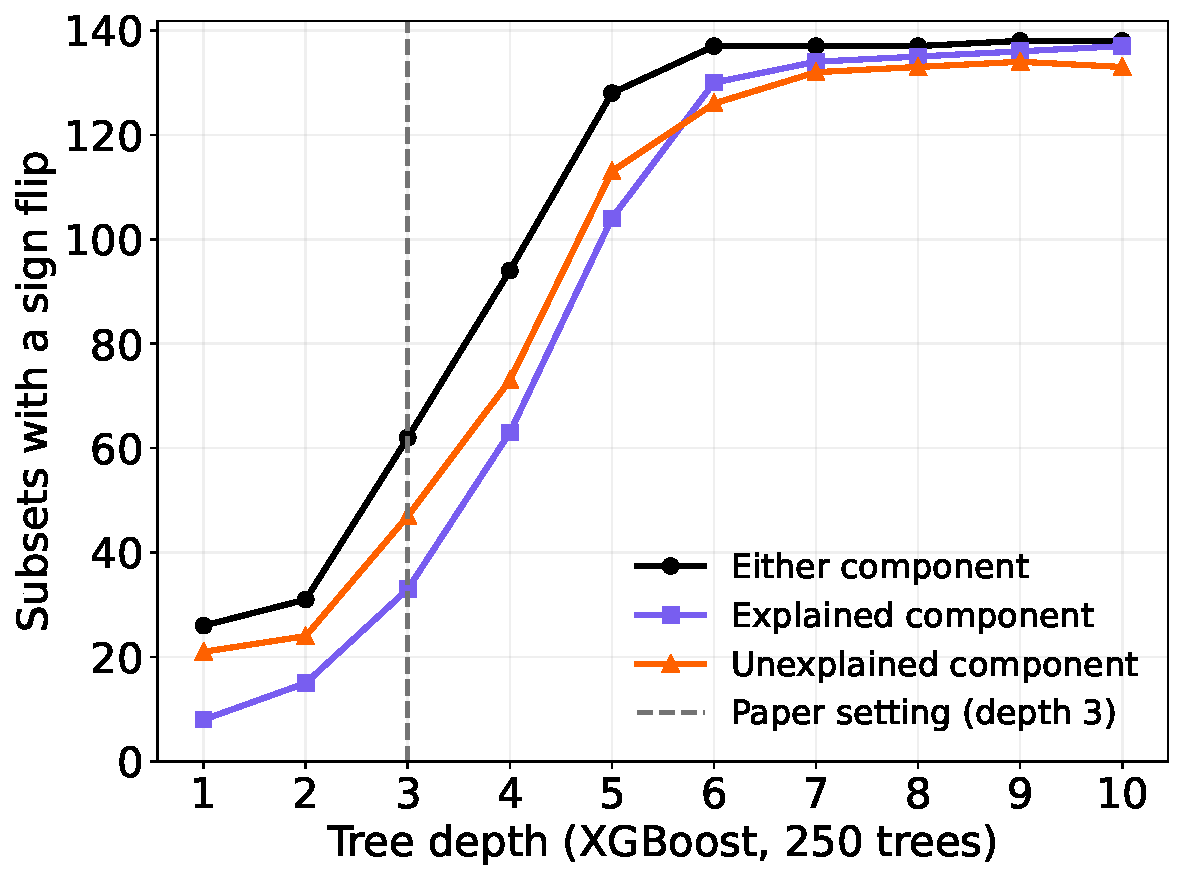
\includegraphics[width=0.3\textwidth]{Sections/Figures/complexity/icu_xgb_depth.pdf}} &
    \raisebox{-0.5\height}{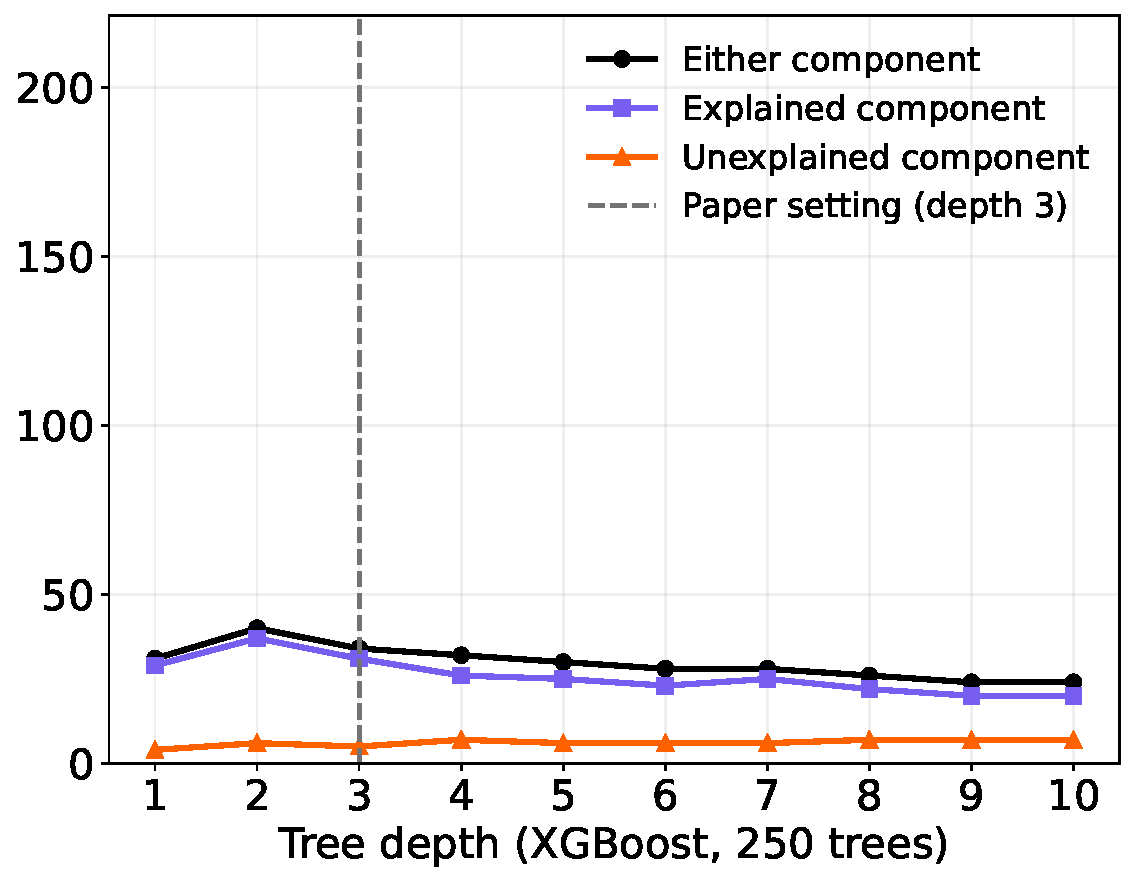
\includegraphics[width=0.3\textwidth]{Sections/Figures/complexity/census_xgb_depth_pincp_noylabel.pdf}} &
    \raisebox{-0.5\height}{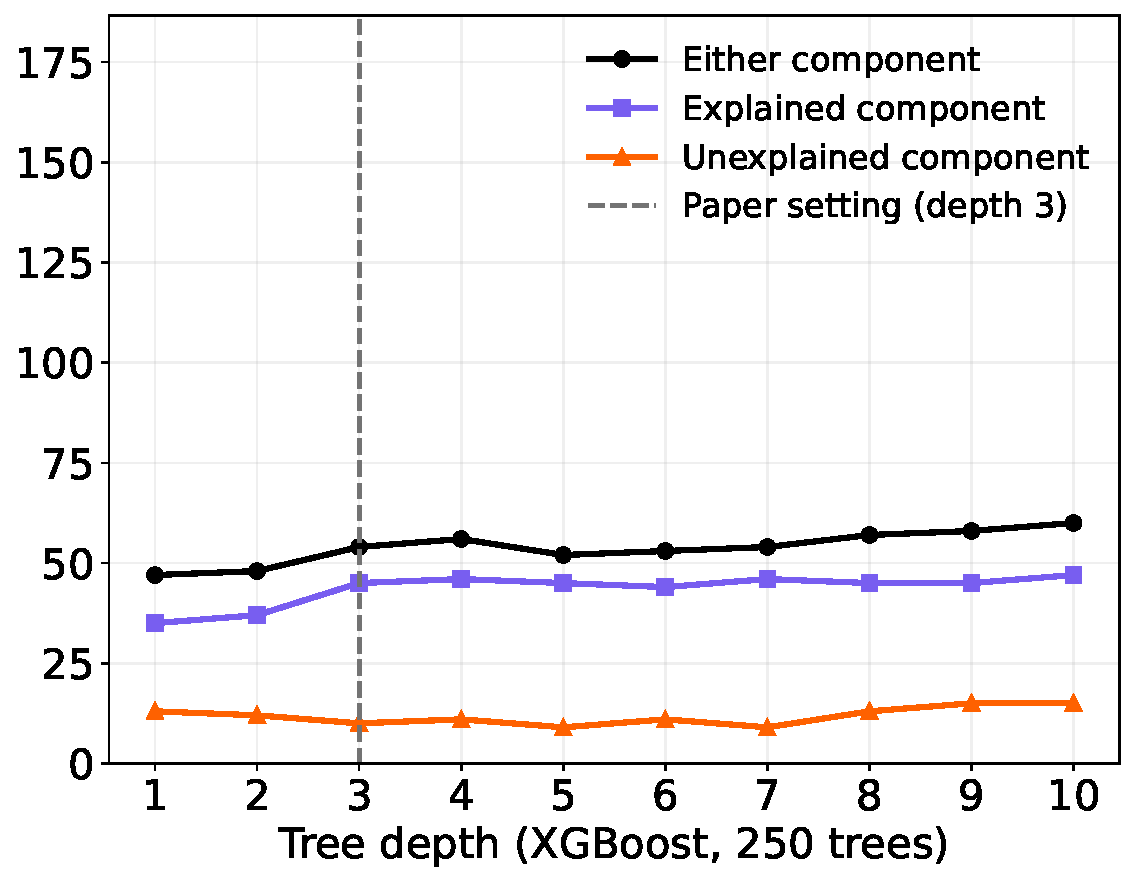
\includegraphics[width=0.3\textwidth]{Sections/Figures/complexity/census_xgb_depth_hicov_noylabel.pdf}} \\[2pt]
    \rotatebox[origin=c]{90}{\small XGBoost: number of trees} &
    \raisebox{-0.5\height}{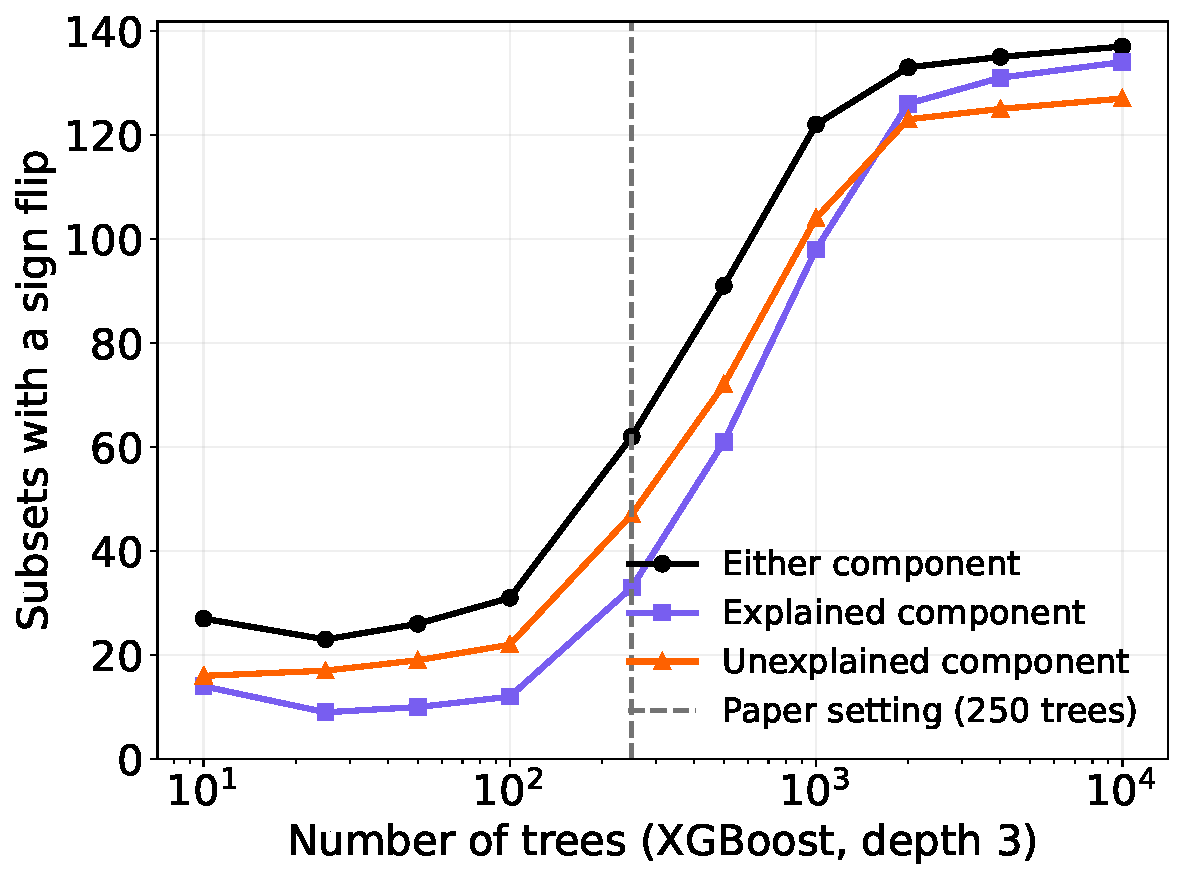
\includegraphics[width=0.3\textwidth]{Sections/Figures/complexity/icu_xgb_trees.pdf}} &
    \raisebox{-0.5\height}{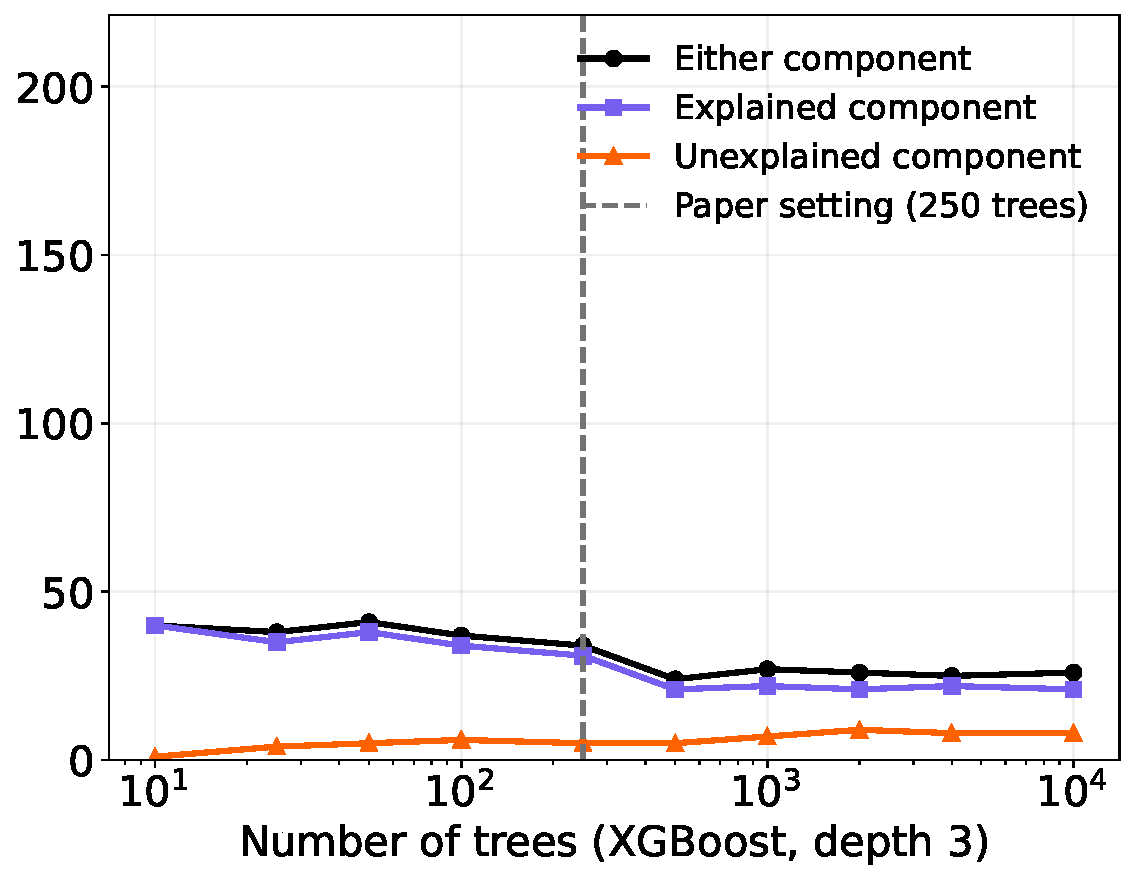
\includegraphics[width=0.3\textwidth]{Sections/Figures/complexity/census_xgb_trees_pincp_noylabel.pdf}} &
    \raisebox{-0.5\height}{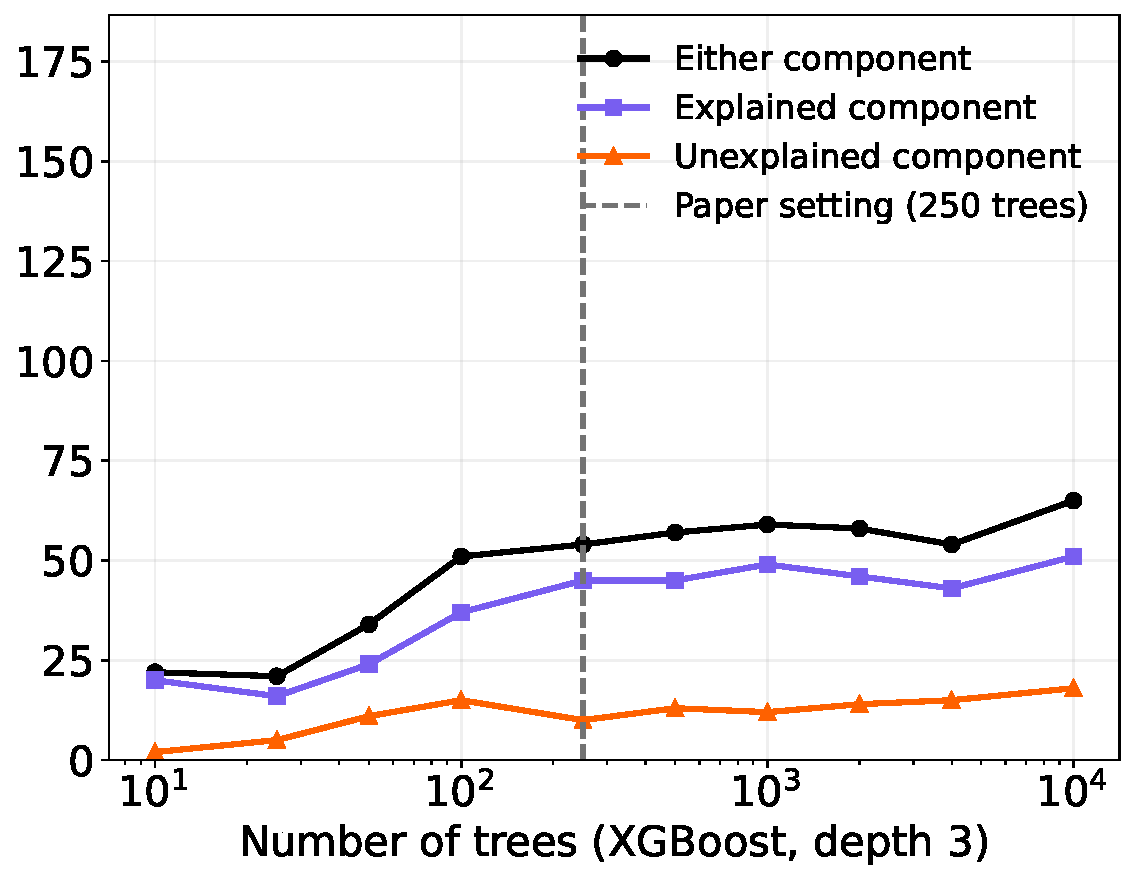
\includegraphics[width=0.3\textwidth]{Sections/Figures/complexity/census_xgb_trees_hicov_noylabel.pdf}} \\[2pt]
    \rotatebox[origin=c]{90}{\small Neural network: width} &
    \raisebox{-0.5\height}{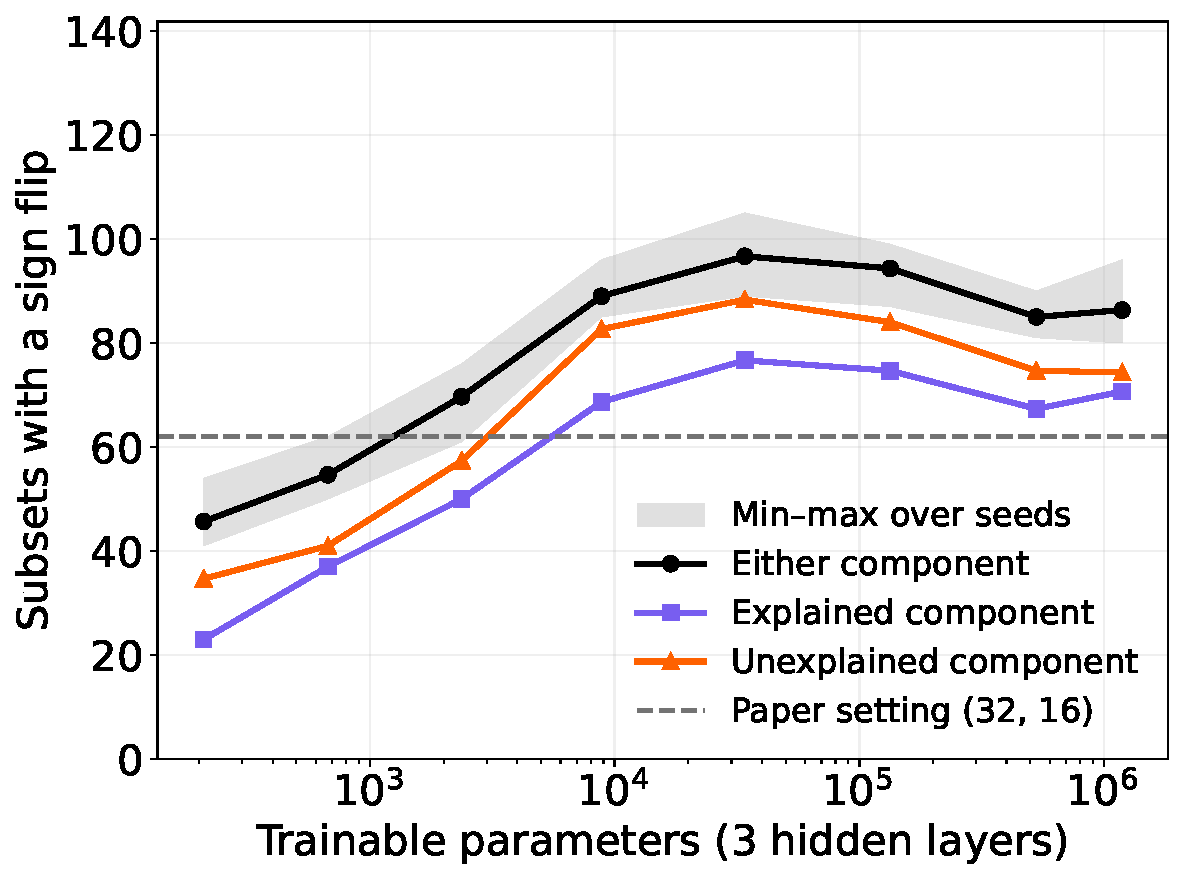
\includegraphics[width=0.3\textwidth]{Sections/Figures/complexity/icu_nn_width.pdf}} &
    \raisebox{-0.5\height}{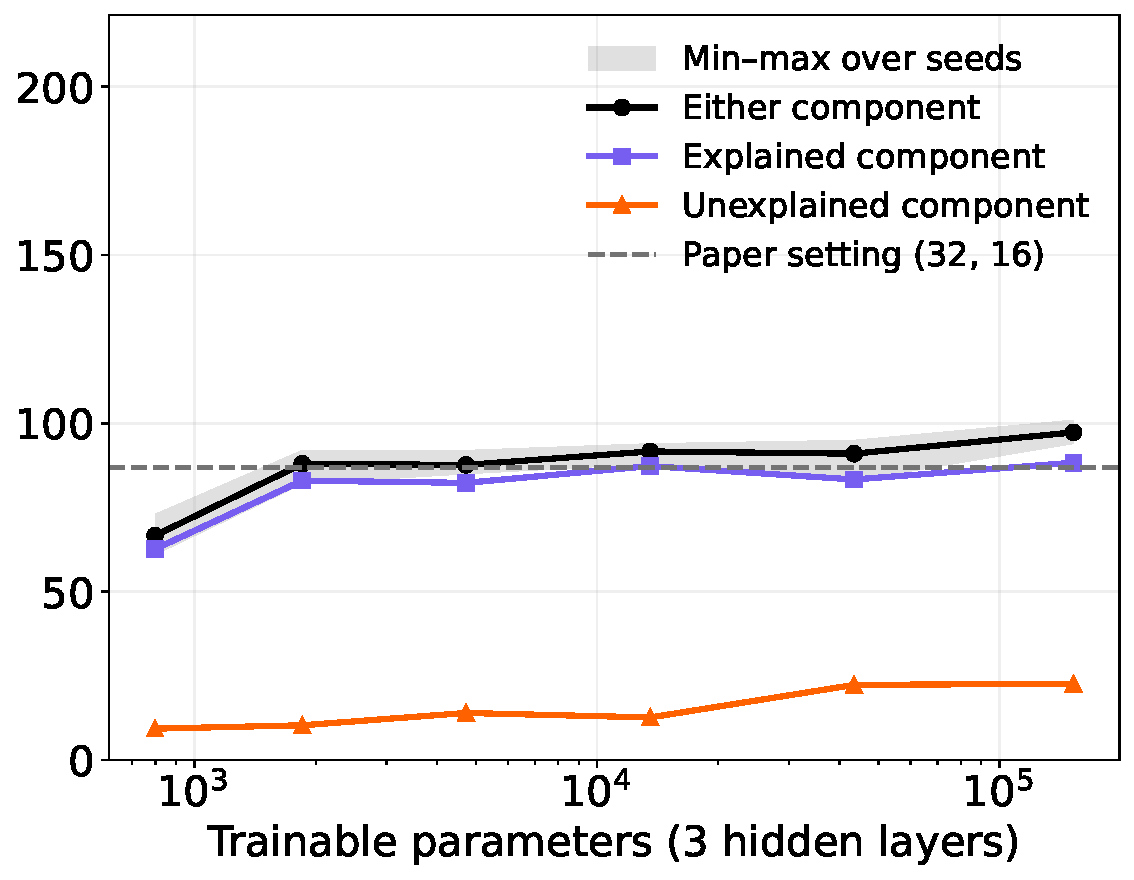
\includegraphics[width=0.3\textwidth]{Sections/Figures/complexity/census_nn_width_pincp_noylabel.pdf}} &
    \raisebox{-0.5\height}{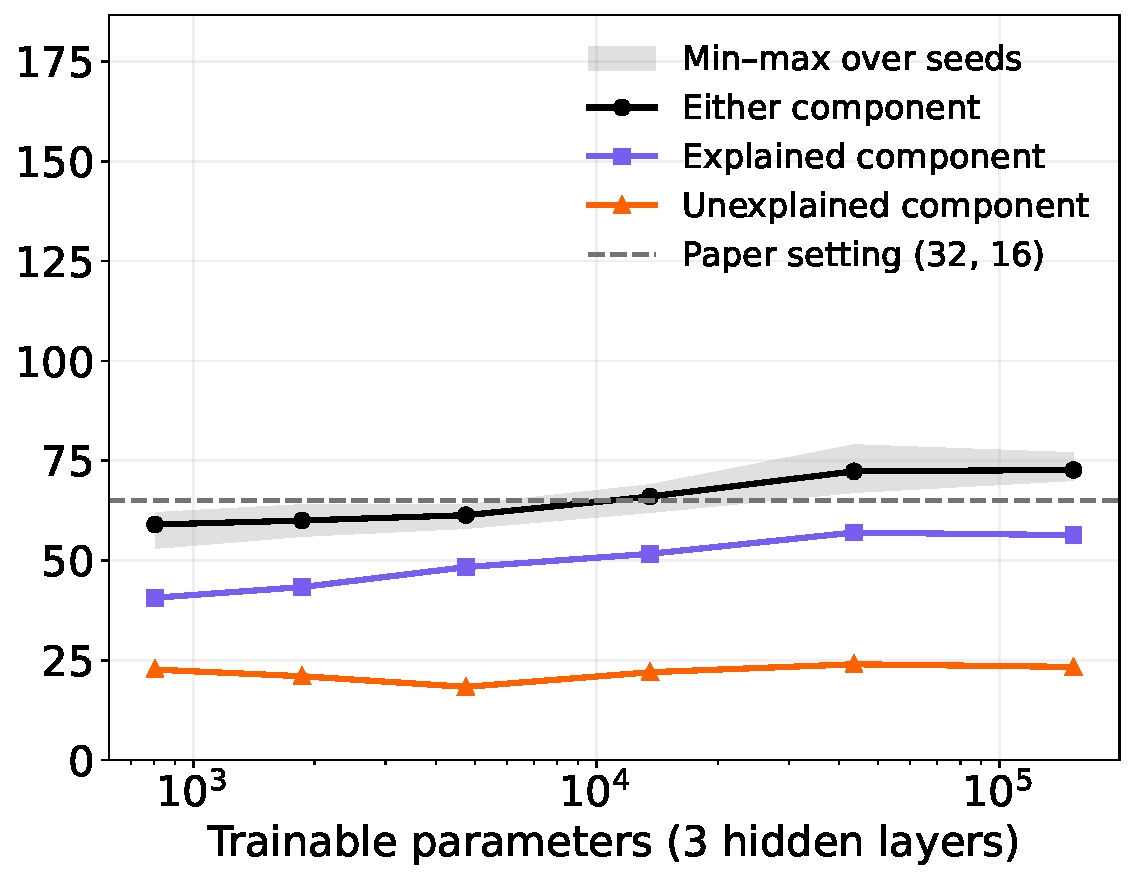
\includegraphics[width=0.3\textwidth]{Sections/Figures/complexity/census_nn_width_hicov_noylabel.pdf}} \\[2pt]
    \rotatebox[origin=c]{90}{\small Neural network: depth} &
    \raisebox{-0.5\height}{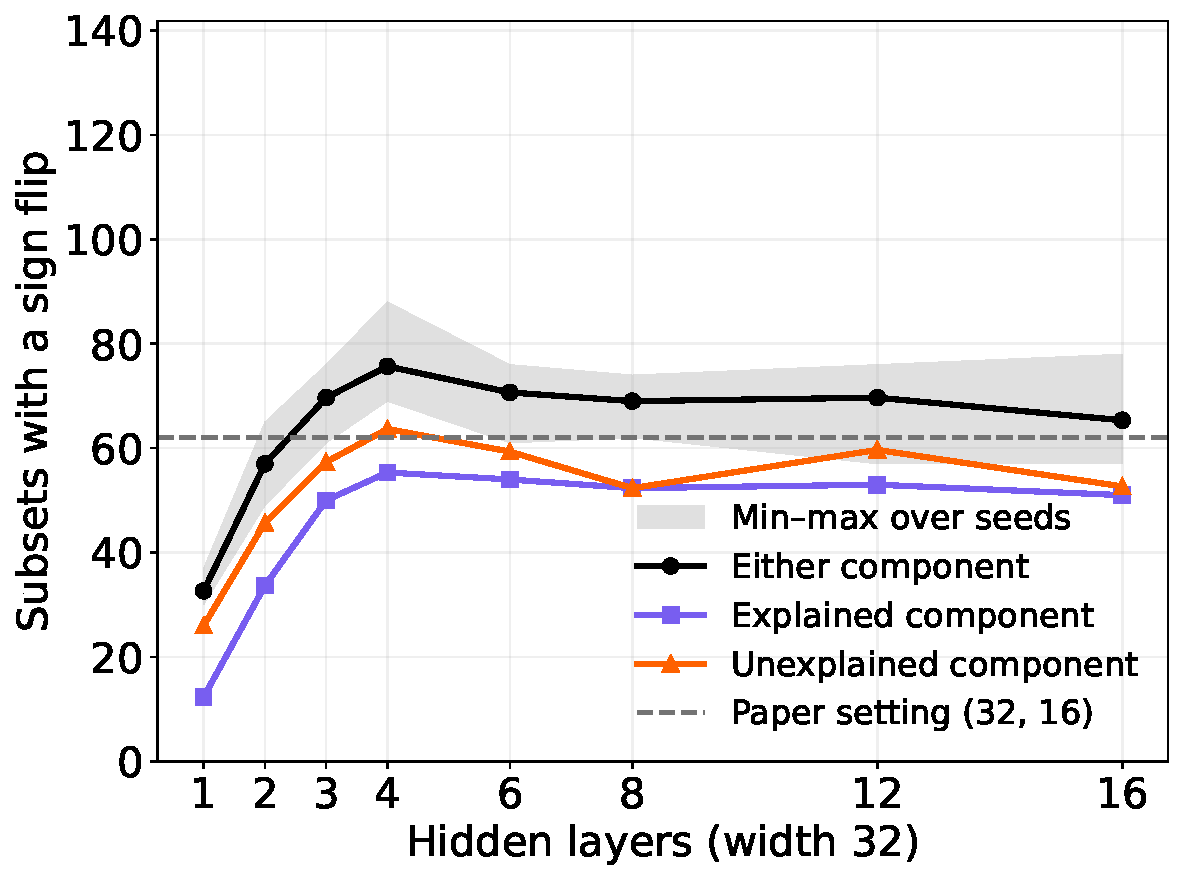
\includegraphics[width=0.3\textwidth]{Sections/Figures/complexity/icu_nn_depth.pdf}} &
    \raisebox{-0.5\height}{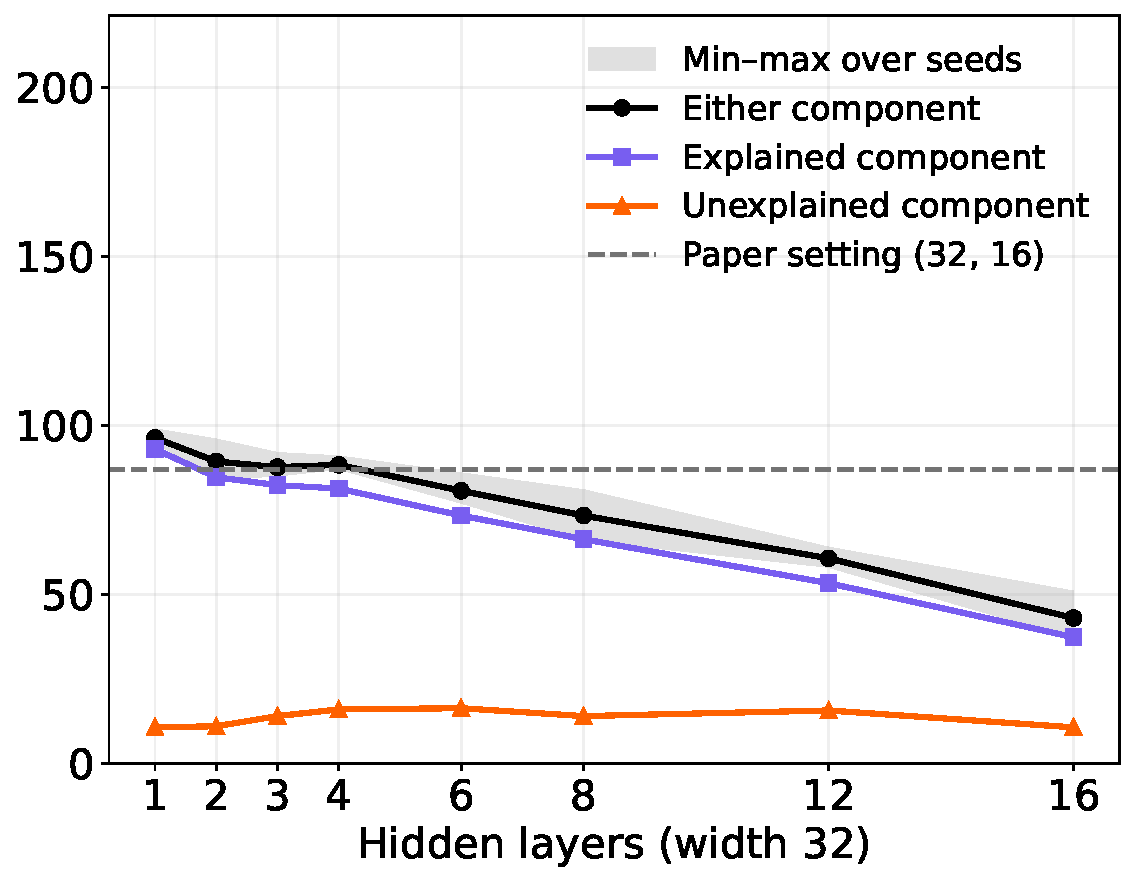
\includegraphics[width=0.3\textwidth]{Sections/Figures/complexity/census_nn_depth_pincp_noylabel.pdf}} &
    \raisebox{-0.5\height}{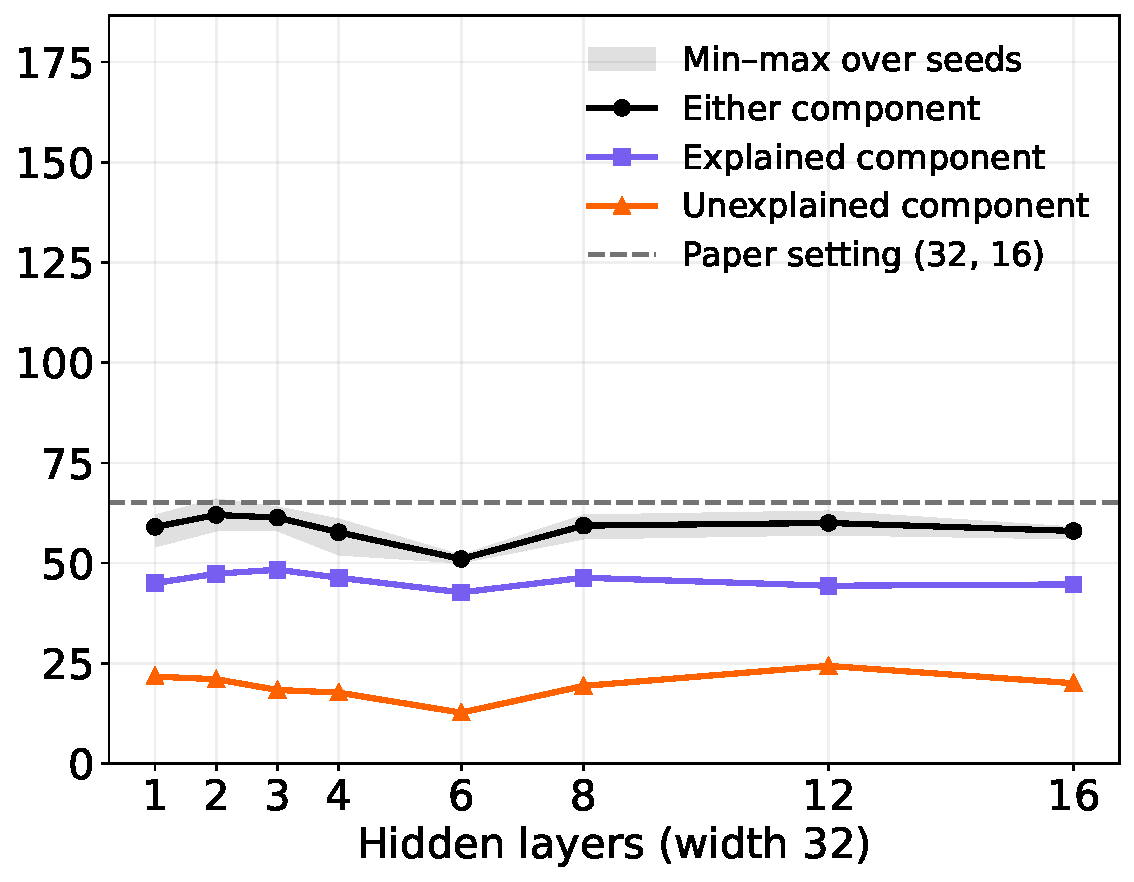
\includegraphics[width=0.3\textwidth]{Sections/Figures/complexity/census_nn_depth_hicov_noylabel.pdf}} \\[2pt]
    \end{tabular}
    \caption{Number of data subsets with a sign flip as a function of model complexity, for the ICU data (left), Census log income (center), and Census health insurance (right). Rows vary the XGBoost tree depth, the XGBoost number of trees, the neural network width (three hidden layers of equal width; horizontal axis is the number of trainable parameters), and the neural network depth (hidden layers of width $32$). Black: either component; purple: explained component; orange: unexplained component. The dashed line marks the setting reported in \cref{tab:flip_summary_main,tab:flips_census_income,tab:flips_census_insurance}. For the neural network, lines are means over three initialization seeds and the shaded band is the range across seeds.}
    \label{fig:complexity_sweeps}
    
\end{figure*}

\section{A simulated example from healthcare}
\label{sec:simulated_example}
The results in \cref{sec:real_example} may raise the question of whether sign reversals are always consequences of model misspecification or sampling variability? 
\cref{sec:signflips} provide theoretical arguments that sign reversals are not, in fact, purely due to misspecification or noise.
We complement those arguments here with a simulated example that exhibits a sign reversal under correct model specification and in population-level parameters.

% To illustrate why \cref{eq:ob_decomp_ref_group} can lead a practitioner to draw substantially different conclusions depending on the reference group used in the OBD, we turn to a simple simulated healthcare example inspired by real-life data.

\textbf{Motivation.}
While our example is purely simulated, it is motivated by the following real-life concerns and observations.
Body mass index (BMI) is a widely recognized and routinely measured marker of wellness \cite{heymsfield2016} and is strongly linked to cardiometabolic outcomes, such as elevated blood pressure \cite{brown2000body}.
A researcher studying cardiac health may use commonly observed covariates like BMI to investigate whether differences in blood pressure between two groups are explainable by differences in basic markers of health between the groups, or differences in how these markers map to blood pressure.

Our example imagines two groups of adults in primary care being followed for elevated blood pressure, using systolic blood pressure (SBP) at a follow-up visit as the outcome $Y$. The BMI ($X$) of each adult is measured at an intake visit.
The first, Group $H$, comes from a higher-resource setting, such as an urban neighborhood with structured care pathways, frequent follow up, and better access to healthy food options. 
The second, Group $K$, comes from a lower-resource setting, where patients face barriers such as longer travel to clinics, infrequent follow up, and limited access to nutritious food.
These factors shape both the composition of each group (including average BMI) and the structure of the SBP--BMI relationship. We follow a clinical literature finding an approximately linear relationship between BMI and SBP \cite{kaufman1997, cappuccio2008, chen2023}; in particular, we assume a separate linear relationship in each group.

While an OBD cannot establish causality without further assumptions, it can suggest where one might look for potential drivers of observed inter-group disparities.
If the explained component is effectively zero and the unexplained component (differences in $Y|X$) dominates (with a sign in the direction of the observed outcome difference), it may highlight the need to investigate differences in medical care, such as adherence support or access to antihypertensives.
If the unexplained component is effectively zero and the explained component (differences in $X$) dominates (with a sign in the direction of the observed outcome difference), it may be most impactful to target interventions on weight management, nutrition, and physical activity. 

\textbf{Simulated data.}
We generate the BMI ($X$, in kg/m$^2$) of an individual in group \( g \) from a group-specific normal distribution.
We simulate \( N = 5000 \) individuals, divided across two groups. Body mass index (BMI) is drawn from normal distributions reflecting realistic population profiles:
\begin{align*}
    \text{BMI}_g &\sim \mathcal{N}(\mu_g ,\, \sigma_g^2) \quad \text{kg/m}^2,
\end{align*}
where \( \mu_H = 25 \), \( \mu_K = 27 \), and \( \sigma_H = \sigma_K = 4 \). Within each group, systolic blood pressure is modeled as a noisy, linear function of BMI:
\begin{align}
    \text{SBP}_g &= \alpha_g + \beta_g \times \text{BMI}_g + \varepsilon_g.
\end{align}
Here $\alpha_g \in \mathbb{R}$ is the group-specific intercept (in units of mmHg); $\beta_g \in \mathbb{R}$ is the group-specific slope, representing the average change in SBP (mmHg) per unit increase in BMI (kg/m$^2$); and $\varepsilon$ reflects individual variability in SBP that is uncorrelated with BMI. We take $\varepsilon$ independent and identically distributed across adult patients, with the same (mean-zero Gaussian) distribution in each group.

The noise term \( \varepsilon_g \) captures unobserved individual-level variation within each group, such as daily measurement fluctuations, dietary salt intake, or transient stress. 
Group~H (higher-resource settings) has a lower mean BMI, consistent with greater access to healthy food, safe environments for physical activity, and preventive care. 
In contrast, Group~K (lower-resource or marginalized settings) has a mean BMI two units higher, reflecting structural disparities related to nutrition, transportation, and economic constraints. 
The shared standard deviation of 4~kg/m\(^2\) reflects typical within-group heterogeneity in adult primary care populations \citep{block2013population}.

We assume \( \beta_K > \beta_H \), reflecting that in Group~K, each additional unit of BMI increases SBP more steeply, due to slower titration, less frequent follow up, greater adherence variability, and fewer lifestyle resources.
In contrast, the flatter slope in Group~H reflects partial buffering through timely medication adjustments, consistent coverage, and access to lifestyle support.
The intercepts \( \alpha_H \) and \( \alpha_K \) are chosen so that the regression lines intersect near the midpoint of the BMI range, ensuring that mean SBP differences are primarily driven by BMI distribution and slope disparity.
\cref{fig:bmi_sbp} shows the fitted linear models to the synthetic data.

\begin{table}[h]
\caption{Key chosen and derived parameters by group. BMI and SBP are in kg/m$^2$ and mmHg respectively. $\alpha$ is in mmHg; $\beta$ is in mmHg per kg/m$^2$.}
\label{tab:dgp_short}
\begin{center}
\small
\begin{tabular}{lcccc}
\toprule
Group & Mean BMI & $\alpha$ & $\beta$ & Mean SBP \\
\midrule
$H$ & 25.0 & 110.4 & 1.0 & 135.4 \\
$K$ & 27.0 & 100.0 & 1.4 & 137.8 \\
\bottomrule
\end{tabular}
\end{center}
\vskip -0.1in
\end{table}

\cref{fig:bmi_sbp} shows the population SBP--BMI relationships for both groups (two lines). The figure also shows data samples
to illustrate the BMI distribution in each group --- as well as how the intercepts, slopes, and BMI distributions interact.
%
Overall, Group $H$ has lower average SBP than Group $K$, owing both to lower average BMI and a shallower slope relating BMI to SBP, perhaps reflecting improved access and adherence to treatment, or availability of non-pharmacological support.
However, Group $H$ has a higher baseline SBP ($\alpha_H$), perhaps reflecting genetic factors in Group $H$.

\begin{figure}[h]
    \centerline{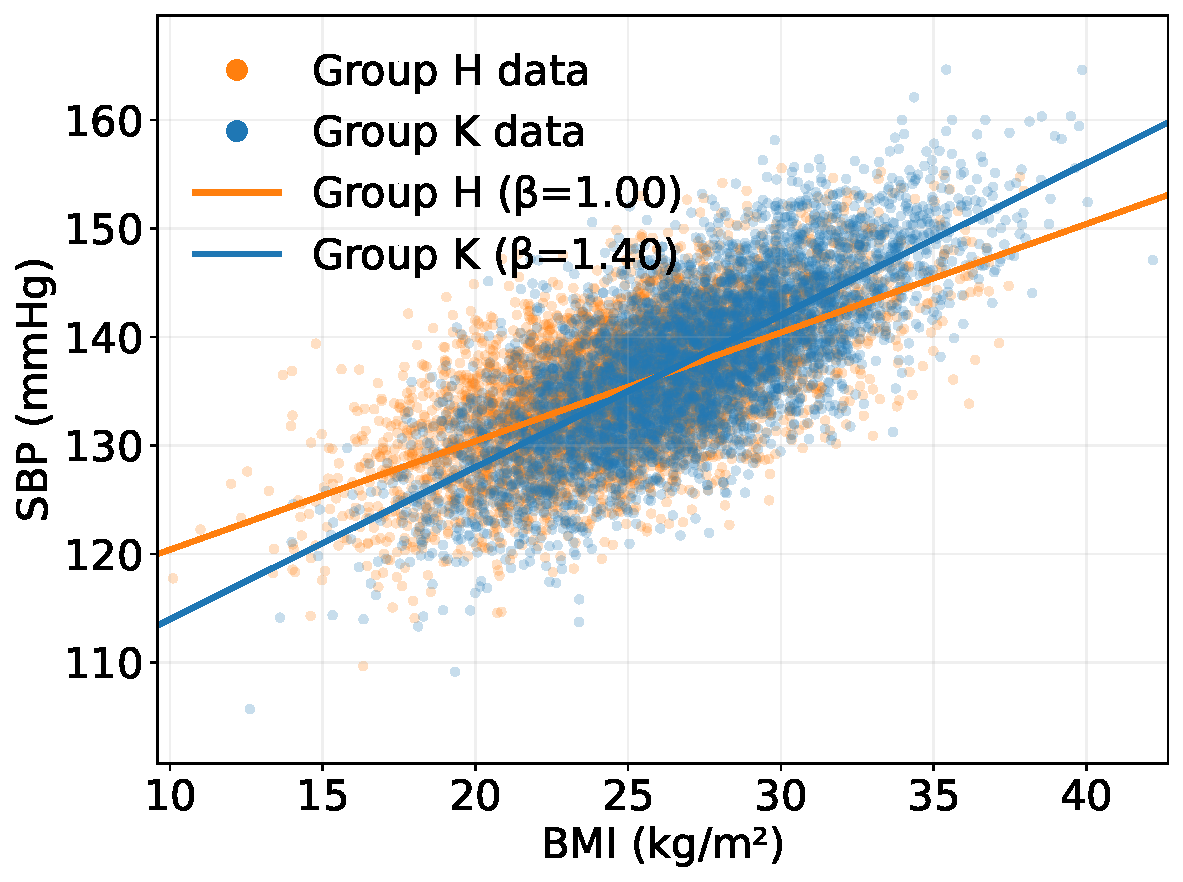
\includegraphics[width=0.42\linewidth]{Sections/Figures/bmi_sbp_comparison_population.pdf}}
\caption{Population linear models of SBP on BMI by group and data samples.}
\label{fig:bmi_sbp}
\end{figure}

\textbf{Analysis.} Since we have access to all population quantities in this example, there is no need to fit models or check statistical significance.
We can compute the OBD directly from the known population distributions.
%In principle, the OBD should provide a transparent framework to separate the difference in mean SBP into an explained component (differences in BMI distribution, $X$) and an unexplained component (differences in SBP given BMI, $Y|X$)

\textbf{Two different conclusions.}
\cref{tab:ob_decomp} summarizes the OBD results under each reference group.
For both choices of reference group the explained components are negative, so both choices of reference imply that $H$'s lower average SBP is due in part to its lower average BMI.
However, the sign of the unexplained OBD component flips depending on the choice of the reference group.
When group $H$ is the reference, the negative unexplained component implies that institutional factors further reduce group $H$'s blood pressure relative to group $K$.
However, when group $K$ is the reference, institutional factors appear to actually \emph{increase} group $H$'s average blood pressure relative to group $K$.
Intuitively, because blood pressure in group $K$ is so much more responsive to BMI, group $H$'s lower average BMI appears so good as to ``over-explain'' the difference in SBP; the unexplained component is then forced to be positive to compensate.

In this example, the sign change is in the unexplained component rather than the explained component (cf.\ \cref{sec:real_example}). Since we simulate the data according to group-specific linear models, there is no misspecification. And since we work directly with population quantities, the difference in OBD conclusions is not a product of sampling error.

\begin{table}[H]
\caption{Population Oaxaca–Blinder decomposition of mean SBP differences. All values are in mmHg.}
\label{tab:ob_decomp}
\begin{center}
\small
\begin{tabular}{lrrr}
\toprule
Reference & Explained & Unexplained & Total gap \\
\midrule
$H$ & $-2.0$ & $\textbf{-0.4}$ & $-2.4$ \\
$K$ & $-2.8$ & $\textbf{0.4}$  & $-2.4$ \\
\bottomrule
\end{tabular}
\end{center}
\vskip -0.1in
\end{table}

% \begin{table}[H]
% \caption{Estimated Oaxaca–Blinder decomposition of mean SBP differences}
% \label{tab:ob_decomp}
% \begin{center}
% \small
% \begin{tabular}{lrrr}
% \textbf{Group} & \textbf{Explained} & \textbf{Unexplained} & \textbf{Total gap} \\
% \hline \\
% H & $-1.91$ & $\textbf{-0.14}$ & $-2.05$ \\
% K & $-2.61$ & $\textbf{0.57}$  & $-2.05$ \\
% \end{tabular}
% \end{center}
% \footnotesize{Note: H = Higher-resource group, K = Lower-resource group. All values in mmHg.}
% \end{table}

%\begin{figure*}[t]
%\vspace{.3in}
%\centerline{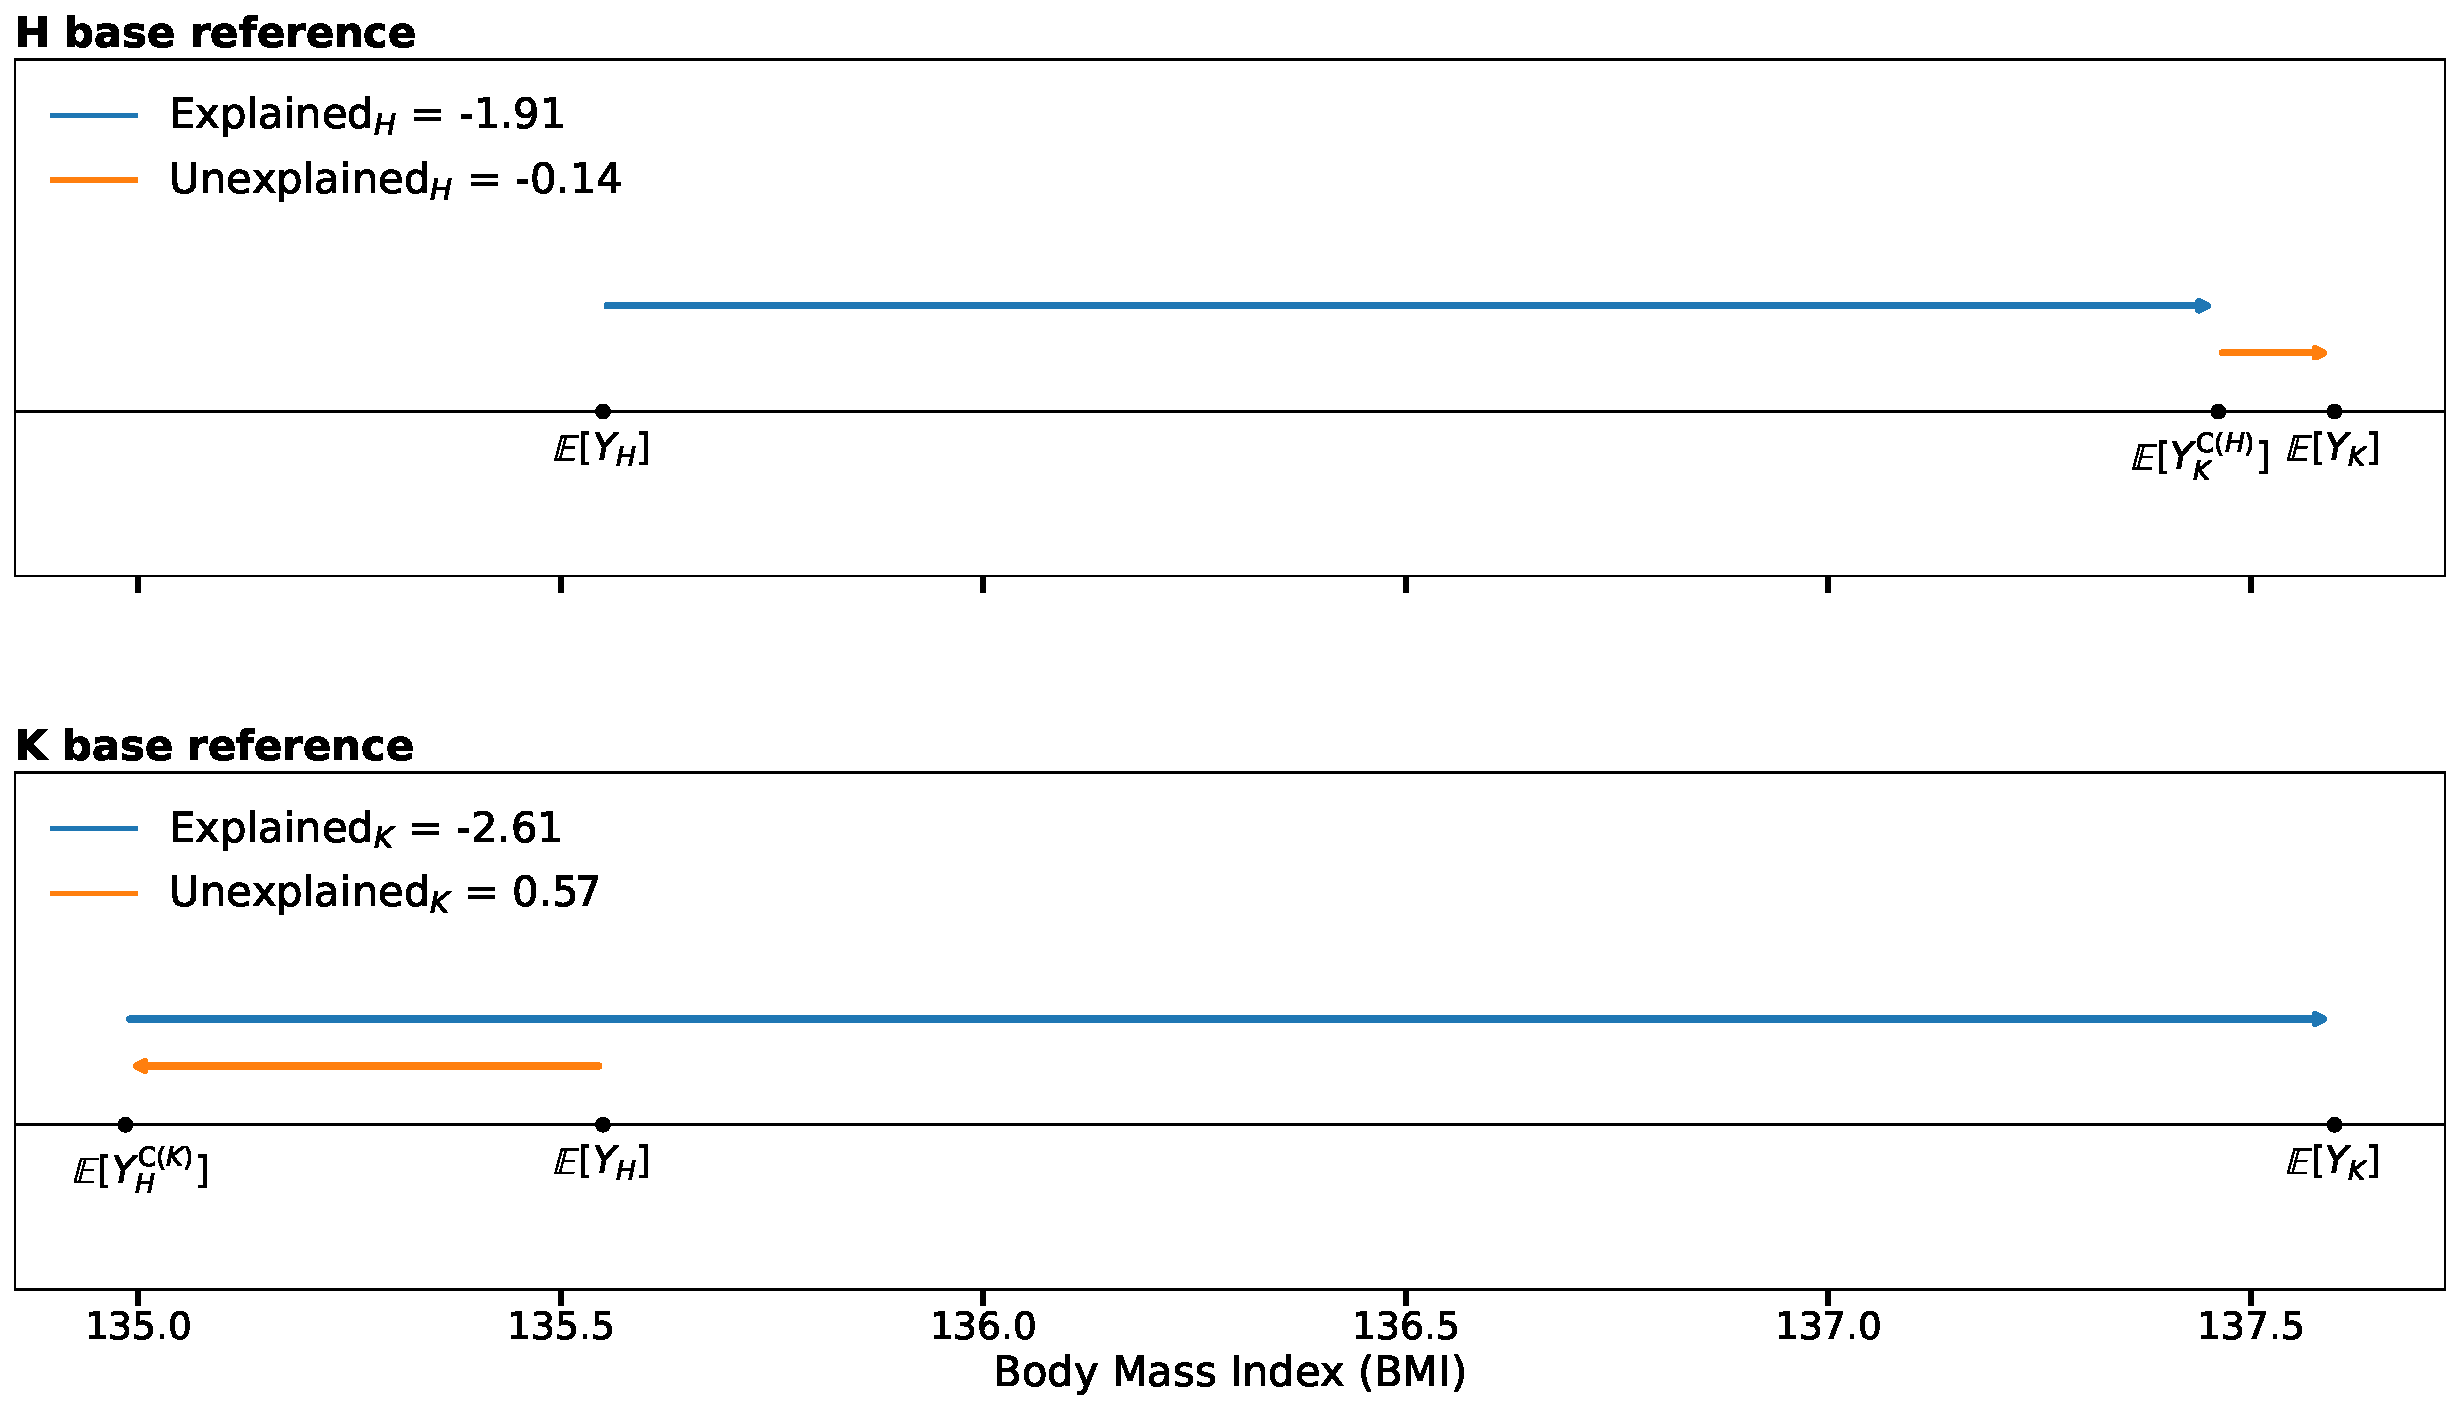
\includegraphics[width=0.7\textwidth]{Sections/Figures/counterfactual.pdf}}
%\vspace{.3in}
%\caption{Counterfactual analysis visualization showing the decomposition results for both reference groups in our simulated example.}
%\label{fig:counterfactual}
%\end{figure*}

%\cref{fig:counterfactual} visualizes the OBD as the mere difference between the counterfactual question posed by each choice of reference group and the observed mean SBP for each group. It also illustrates the sign flip in the unexplained component.

% mega double check conclusion:
% Some authors might argue that the choice of reference group simply reflects a different counterfactual question, for example, ``What would the SBP gap be if the lower resource group had the BMI--SBP relationship of the higher resource group?'' versus ``What would the gap be if the higher resource group had the BMI--SBP relationship of the lower resource group?'' 
% Others might claim that the true effect lies somewhere between these two extremes, and that averaging across reference groups provides a balanced view. 
% However, in our setting we argue that such sensitivity is problematic: when the sign of the unexplained component reverses, the qualitative policy message changes, creating a real risk of misinterpretation rather than a benign difference in framing.



\section{Theory}
\label{app:theory}

\subsection{Proof of \cref{prop:generic_flip_probs}}
\label{app:proof_generic_flip_probs}

\begin{proof}
	For ease of notation, define $\E(f) := V(f) - W(f)$. We have that the probability of an explained flip is equal to:
	\begin{equation*}
		Pr\bigg( \{\E(f^H) < 0, \E(f^K) > 0 \} \cup \{ \E(f^H) > 0, \E(f^K) < 0\} \bigg).
	\end{equation*}
	The two events in the union are disjoint, and, because $f^H, f^K$ are i.i.d.\, the events have equal probability. So we have:
	\begin{align*}
		&= 2 Pr\bigg( \{\E(f^H) < 0, \E(f^K) > 0 \} \bigg) \\
		&= 2 Pr\bigg( \E(f^H) > 0 \bigg) Pr\bigg( \E(f^K) < 0 \bigg) \\
		&= 2 q (1 - q),
	\end{align*}
	where we have used that $f^H, f^K$ are i.i.d.\ and that $\nu(\E = 0) = 0$.
	
	For the unexplained component, we have that there is a sign flip if and only if the product of the two unexplained components is negative. By definition, this is equivalent to $(V - V')(W - W') < 0$.
\end{proof}

\subsection{Lemmas for the proof of \cref{prop:sign_flip_gp}}

We need a few lemmas before proving \cref{prop:sign_flip_gp}.

\begin{lemma} \label{lem:bivariate_product}
Assume that for random variables $A, B$, we have that $(A,B)$ is a bivariate normal with:
\begin{equation}
\begin{pmatrix} A \\ B \end{pmatrix} \sim
N \left( 
		\begin{pmatrix} \mu_A \\ \mu_B \end{pmatrix},
		\begin{pmatrix} \sigma_A^2, & \rho \sigma_A \sigma_B \\ \rho \sigma_A \sigma_B & \sigma_B^2 \end{pmatrix}
\right).
\end{equation}
Then it holds
\begin{equation}
	Pr(AB < 0) = \Phi(\mu_A / \sigma_A) + \Phi(\mu_B / \sigma_B) - 2 \Phi_{biv}(\mu_A / \sigma_A, \mu_B / \sigma_B, \rho),
\end{equation}
where $\Phi$ is the CDF of a standard normal distribution, and $\Phi_{biv}$ is the CDF for a standard bivariate normal distribution.\footnote{For a bivariate Gaussian $(A,B)$ with unit standard deviations and correlation coefficient $\rho$, we have $\Phi_{biv}(a,b,\rho) := \int_{-\infty}^a \int_{-\infty}^b \phi_{biv}(x, y; \rho) dx dy$, where $\phi_{biv}(\cdot, \cdot;\rho)$ is the pdf of a standard bivariate normal.}
\end{lemma}
\begin{proof}
	We have that:
	\begin{align*}
		& Pr(A > 0) = Pr(A > 0, B < 0) + Pr(A > 0, B > 0) \\
		& Pr(B > 0) = Pr(A < 0, B > 0) + Pr(A > 0, B > 0).
	\end{align*}
	Now, noting that $Pr(AB < 0) = Pr(A > 0, B < 0) + Pr(A < 0, B > 0)$ and adding the above two equations together, we have that:
	\begin{equation*}
		Pr(A > 0) + Pr(B > 0) = Pr(AB < 0) + 2Pr(A > 0, B > 0).
	\end{equation*}
	Now, if $Z$ is a standard normal, then we have that $Pr(A > 0) = Pr(\mu_A + \sigma_A Z > 0) = \Phi(\mu_A / \sigma_A)$. Similar logic applied to the other probabilities in the above equation completes the proof.
\end{proof}

\begin{lemma} \label{lem:vw_bivariate}
	Take \cref{assum:iid,assum:atomless,assum:gp,assum:fubini}. Then $(V(f), W(f))$ is a bivariate normal with:
	\begin{align}
		& \mu_V = \int \mu(x) h(x) dx, \quad \mu_W = \int \mu(x) k(x) dx \\
		& \sigma_V = \| h \|_C, \quad \sigma_W = \| k \|_C, \quad \rho = \frac{<h,k>_C}{\| h \|_C \| k \|_C}.
	\end{align}
\end{lemma}
\begin{proof}
For the means, \emph{if} we are able to exchange the order of integrals, then we can compute $E_f[V(f)] = E_f [ \int f(x) h(x) dx] = \int \mu(x) h(x) dx$, and likewise for $W$.
We now show that we can exchange the order of integrals.
First, note that for $f \sim GP(\mu, C)$, we have that for any $x$, $E_f [|f(x)|] = E_Z [| \mu(x) + \sqrt{C(x,x)} Z|]$, where $Z \sim N(0,1)$. Then $E_f [|f(x)|] \leq |\mu(x)| + \sqrt{C(x,x)} \sqrt{2/\pi}$.
Therefore,
\begin{equation}
	E_f \left[ \int |f(x)| h(x) dx \right] \leq E_f \left[ \int | \mu(x) | h(x) dx + \int \sqrt{C(x,x)} \sqrt{\frac{2}{\pi}} h(x) dx \right],
\end{equation}	
which is finite by \cref{assum:fubini}. Thus by Fubini's theorem, we have $E_f [ \int f(x) h(x) dx] = \int \mu(x) h(x) dx$ as claimed.
For the variances, it is easier to work with $\bar f := f - \mu$.
We will again first assume that the order of integrals can be exchanged and then prove that this is allowable.
\begin{align*}
	Var[V(f)] &= Var[V(\bar f)] = E \left[ \left( \int \bar f(x) h(x) dx \right)^2 \right] \\
	&= E \left[ \left(\int \bar f(x') h(x') dx' \right) \left( \int \bar f(x) h(x) dx \right) \right] \\
	&= \int\int E[ \bar f(x') \bar f(x)] h(x) h(x') dx' dx \\
	&= \int\int C(x,x') h(x) h(x') dx' dx = \| h \|_C^2.
\end{align*}
To see that the above exchange of integrals is allowed, note that, by Cauchy-Schwarz applied to $E_f[ \bar f(x') \bar f(x)]$, we have:
\begin{align*}
	\int\int E_f[ \bar f(x') \bar f(x)] h(x) h(x') dx' dx &\leq \int\int \sqrt{E_f[ f(x)^2] E_f[f(x')^2]} h(x) h(x') dx dx' \\
	&= \int\int \sqrt{C(x,x) C(x',x')} h(x) h(x') dx dx.
\end{align*}
By \cref{assum:fubini}, this last integral is finite.
Thus, as claimed, $E \left[ \left(\int \bar f(x') h(x') dx' \right) \left( \int \bar f(x) h(x) dx \right) \right] = \int\int E[ \bar f(x') \bar f(x)] h(x) h(x') dx' dx$.

Finally, to compute the correlation coefficient, note that the covariance of $V$ and $W$ is given by:
\begin{align*}
	Cov[ V( \bar f), W(\bar f) ] = \int\int C(x,x') h(x) k(x') dx' dx = \langle h, k \rangle_C.
\end{align*}
This also requires an exchange of integrals which likewise holds by Fubini's theorem and \cref{assum:fubini}. Noting that the correlation coefficient of a bivariate normal is given by its covariance divided by each standard deviation completes the proof.
\end{proof}

\subsection{Proof of \cref{prop:sign_flip_gp}}
\label{app:proof_sign_flip_gp}

Now we can prove \cref{prop:sign_flip_gp}.
\begin{proof}
We prove the unexplained and explained components separately.

	\paragraph{Unexplained component.} We first show the probability of an unexplained sign flip. 
	Let $(V_1, W_1)$ and $(V_2, W_2)$ be i.i.d.\ copies of the pair $V,W$; by \cref{lem:vw_bivariate}, these are i.i.d.\ draws from a bivariate normal.
	Now, the two unexplained components are equal in distribution to $(V_1 - V_2, W_1 - W_2)$.
	This tuple is also a bivariate normal, and has mean zero, $Var[V_1 - V_2] = 2 \| h \|^2_C$, $Var[W_1 - W_2] = 2 \| k \|_C^2$, and $Cov[V_1  - V_2, W_1 - W_2] = 2 \langle h, k \rangle_C$.
	We can then apply \cref{lem:bivariate_product} to get:
	\begin{align}
		Pr[\mathrm{unexplained\ sign\ flip}] &= Pr[ (V_1 - V_2) (W_1 - W_2) < 0] \\
		&= \Phi(0) + \Phi(0) - 2\Phi_{biv}(0,0,\rho),
	\end{align}
	where $\rho = 2\langle h,k \rangle_C / (2 \|h\|_C \|k\|_C$).
	First, we have that $\Phi(0) = 1/2$.
	Next, we have that $\Phi_{biv}(0,0,\rho) = 1/4 + \arcsin(\rho) / (2\pi) = 1/2 - \arccos(\rho) / (2\pi)$ \citep[Eq.\ (69)]{weisstein2026bivariate}.
	So:
	\begin{equation}
		Pr[\mathrm{unexplained\ sign\ flip}] = \frac{1}{\pi} \arccos(\rho) = \frac{1}{\pi} \arccos\left(\frac{\langle h, k \rangle_C}{\| h \|_C \| k \|_C} \right).
	\end{equation}
	
	\paragraph{Explained component.} The explained component is equal to $V(f) - W(f)$, which is normally distributed with mean $\mu_V - \mu_W$ and variance $\sigma_E^2 := \| h \|_C^2 + \| k \|_C^2 - 2\rho \| h \|_C \| k \|_C$. 
	By \cref{prop:generic_flip_probs}, we just need to compute the probability $q := Pr[V(f) - W(f) > 0]$, and then the probability of a sign flip is $2 q (1-q)$.
	We have that $q = \Phi((\mu_V - \mu_W) / \sigma_E)$. 
	Noting that $\sigma_E = \| h - k \|_C$ and that $\mu_V - \mu_W = \int \mu(x) h(x) dx - \int \mu(x) k(x) dx = \langle h-k, \mu \rangle$, we have that $q = \Phi(\lambda)$ for $\lambda := \langle h-k, \mu \rangle / \| h - k \|_C$.
	Using $1-q = \Phi(-\lambda)$ gives:
	\begin{equation}
		Pr[\mathrm{explained\ sign\ flip}] = 2 \Phi(\lambda) \Phi(-\lambda).
	\end{equation}
	
	

\end{proof}


\section{Unbounded sensitivity at fixed mean gap}
 \label{ex:unbounded}
In this section we present a toy example where we can have arbitrarily large flip magnitudes. Consider the following example. Assume we have a parameter \( L > 0 \) which controls the magnitude of the covariate shift, and \( \varepsilon > 0 \) which controls the deviation in slope coefficients. We assume the mean vector is given by \( (\mu_K, \mu_H) = (0, L) \), and the slope parameters deviate symmetrically from \( \frac{1}{L} \), so that \( \beta_H = \frac{1}{L} + \frac{\varepsilon}{2} \), \( \beta_K = \frac{1}{L} - \frac{\varepsilon}{2} \), and the intercepts satisfy \( \Delta\alpha = \alpha_H - \alpha_K = -\frac{L\varepsilon}{2} \), so that \( \Delta_Y = 1 \). Then, the explained and unexplained components under both reference groups are:
% two-column layout: one component per line (layout only). %REV: originally E and U of each reference shared a line.
\begin{align*}
    E^{(H)} &= \Delta\mu \cdot \beta_H = L\left(\frac{1}{L} + \frac{\varepsilon}{2}\right) = 1 + \frac{L\varepsilon}{2}, \\
    U^{(H)} &= \Delta\alpha + {} \mu_K \cdot \Delta\beta = -\frac{L\varepsilon}{2}, \\
    E^{(K)} &= \Delta\mu \cdot \beta_K = L\left(\frac{1}{L} - \frac{\varepsilon}{2}\right) = 1 - \frac{L\varepsilon}{2}, \\
    U^{(K)} &= \Delta\alpha + {} \mu_H \cdot \Delta\beta = +\frac{L\varepsilon}{2}.
\end{align*}

Hence, the difference between the two explained components is \( E^{(H)} - E^{(K)} = L\varepsilon \), which can be made arbitrarily large as \( L \to \infty \), even though the total mean gap is always fixed at \( \Delta_Y = 1 \). Similarly, the unexplained components differ by \( U^{(K)} - U^{(H)} = L\varepsilon \).

\begin{center}
\begin{tabular}{ccccccc}
\toprule
\(L\) & \(\varepsilon\) 
& \(E^{(H)}\) & \(E^{(K)}\) 
& \(U^{(H)}\) & \(U^{(K)}\) 
& Flip? \\
\midrule
20    & 0.1  & \(2\)     & \(0\)      & \(-1\)    & \(1\)     & \checkmark \\
200   & 0.1  & \(11\)    & \(-9\)     & \(-10\)   & \(10\)    & \checkmark \\
1000  & 0.1  & \(51\)    & \(-49\)    & \(-50\)   & \(50\)    & \checkmark \\
\bottomrule
\end{tabular}
\end{center}

Note that the sign flip is symmetric by construction, but the magnitude of the discrepancy grows linearly in \( L \), highlighting that the attribution gap between reference groups can be stretched arbitrarily far.

\section{Why Are Multiple Testing Corrections Irrelevant?}
\label{app:multiple_testing}
The main issue is that we're asking a different question in this paper than the question a multiple testing correction answers. 
In \cref{tab:flip_summary_main}, we are essentially computing a failure rate for a particular subset of analyses using the OBD.
For this subset of analyses, we ask: how often does the OBD, performed at typical significance thresholds, return conflicting conclusions depending on the reference group? 
Each analysis in the ICU mortality, Census log income, and Census insurance examples is one trial of that procedure, and we report the number of trials that ``fail'' (i.e., return conflicting conclusions, making them index ambiguous). A multiple testing correction is not necessary for this argument.

A useful analogy is reliability testing for mechanical parts. An industrial statistician who tests a machine part in 500 different environments and observes 50 failures would report a 10\% failure rate. We would not ask this statistician to apply a multiple testing correction for having conducted 500 trials. In fact, doing so would dilute the estimated failure rate towards zero as the testing program grows more comprehensive.
This is because multiple testing corrections, like the Bonferroni or Holm procedures, control false rejection rates across a family of tests. 
However, measuring a failure rate is a \textit{single test} with \textit{many trials}; there is no ``family'' of tests to correct for.

\textbf{Illustrative Example.}
To be more precise, consider the following stylized example. Suppose we have a population of data analyses where, by construction:
\begin{itemize}
\item The OBD with linear regression always gives an unexplained component of exactly 0 for both reference groups.
\item The OBD with TabPFN always gives $-1$ under one reference group and $+1$ for the other, with a standard error of 0.4.
\end{itemize}
Then, TabPFN will produce index ambiguity at the 5\% level in every analysis, and linear regression never does.
These rates are ground truth for this hypothetical population.

Now, suppose we sampled $N$ analyses from this population and wanted to estimate the rate of index ambiguity at the 5\% level.

First, we could count how many sign flips were significant at the 5\% level. 
TabPFN would report index ambiguity $N/N$ cases versus $0/N$ for linear regression.
So, raw counts (which we report in the paper) reflect ground truth.

Second, we could count how many sign flips were significant at a level adjusted for multiple testing.
For example, under a Bonferroni correction, we would report the number of analyses significant at the $\alpha / N$ level.
With even $N = 10$ analyses this threshold would be $0.005$, and no TabPFN sign flip would survive this test.
We would then report $0/N$ flips for both methods, which is the wrong conclusion.
Other multiple hypothesis corrections (which set more severe thresholds for some of the tests) would have similar problems.
So it is incorrect to use multiple hypothesis testing here.
\section{Licenses of software assets}
\label{appendix:licenses}

Below we list all libraries and packages used in our code, along with the version pinned during our experiments and the corresponding license.

\begin{itemize}
    \item \texttt{numpy==1.26.*} --- BSD 3-Clause License
    \item \texttt{pandas==2.2.*} --- BSD 3-Clause License
    \item \texttt{scipy==1.13.*} --- BSD 3-Clause License
    \item \texttt{scikit-learn==1.5.*} --- BSD 3-Clause License
    \item \texttt{statsmodels==0.14.*} --- BSD 3-Clause License
    \item \texttt{matplotlib==3.8.*} --- BSD 3-Clause License
    \item \texttt{xgboost==2.1.*} --- Apache License 2.0
    \item \texttt{joblib==1.4.*} --- BSD 3-Clause License
    \item \texttt{tabpfn==2.0.*} --- Custom license: \url{https://huggingface.co/Prior-Labs/tabpfn_2_6/blob/main/LICENSE}
\end{itemize}

Our code also uses R version 4.5.2 (License: GNU GPL version 2); the replication code lists all used R software packages, versions, and licenses in the `renv.lock' file.
